% Generated from the shared content.py source; edit that source for synchronized editions.
% Compile with XeLaTeX (twice), or Tectonic.
\documentclass[UTF8,fontset=fandol,12pt]{ctexart}
\usepackage{graphicx,amsmath,amssymb,booktabs,longtable,array,geometry,fancyhdr,setspace,url,needspace}
\usepackage[hidelinks,unicode]{hyperref}
\geometry{a4paper,top=25.4mm,bottom=25.4mm,left=31.75mm,right=31.75mm,headheight=15pt,headsep=10mm,footskip=9mm}
\onehalfspacing
\setlength{\parindent}{2em}
\setlength{\parskip}{0pt}
\setlength{\tabcolsep}{4pt}
\renewcommand{\arraystretch}{1.25}
\setlength{\LTpre}{6pt}
\setlength{\LTpost}{6pt}
\setlength{\emergencystretch}{2em}
\clubpenalty=10000
\widowpenalty=10000
\hbadness=10000
\ctexset{section={format=\bfseries\heiti\fontsize{14}{21}\selectfont,beforeskip=16pt,afterskip=10pt},subsection={format=\bfseries\heiti\fontsize{12}{18}\selectfont,beforeskip=12pt,afterskip=6pt},subsubsection={format=\bfseries\fontsize{12}{18}\selectfont,beforeskip=10pt,afterskip=5pt}}
\pagestyle{fancy}
\fancyhf{}
\fancyfoot[C]{\fontsize{10.5}{13}\selectfont\thepage}
\renewcommand{\headrulewidth}{0.4pt}
\fancypagestyle{firstpage}{\fancyhf{}\renewcommand{\headrulewidth}{0pt}\fancyfoot[C]{\fontsize{10.5}{13}\selectfont\thepage}}
\urlstyle{same}
\begin{document}
\special{pdf:minorversion 7}
\thispagestyle{firstpage}
\begin{center}

\includegraphics[width=11.5cm]{images/contest_logo.png}
\end{center}
\vspace{8pt}
\begin{center}{\heiti\bfseries\fontsize{18}{27}\selectfont PMUX结构优化与逻辑零初态验证系统\par}\end{center}
\Needspace{129.6pt}\section*{摘要}
针对PMUX与算术、状态控制交织时共享结构难以保留的问题，本作品在Yosys中实现内置C++优化pass，并在原synth\_\allowbreak{}intel流程中完成初始化声明与词级重构。初始化阶段紧接proc，在顺序优化及状态重编码前把未指定时钟触发器初值声明为逻辑0，保留显式0/\allowbreak{}1；受支持可写RAM仅补充未定义存储位，纯ROM内容不改。重构阶段结合精确控制恢复、多层数据通路、bank、全字算术、闭合选择DAG及有界小ROM共享；进一步联合使能约束下的状态投影与公共译码因子，并重述PMUX采样边界的同步复位与使能优先级，保留原状态转移，在显式Cyclone IV目标下映射硬件同步清零并编码已知初值；并将已证互斥的叶分支迁移到SLOAD/\allowbreak{}ASDATA；后续标准流程与ABC9保持不变。r30\_\allowbreak{}native\_\allowbreak{}sload保持原4例及新增5例的源文件、默认参数和外部脚本不变；LUT+NOT逐例不增，缩减率算术平均36.2522\%，总量2427\ensuremath{\rightarrow}1482。在v3 两命令范围内，综合时间比与主进程峰值工作集比逐例均不超过1.05。完整EQY从原RTL的明确逻辑零初态出发，证明到候选实际默认综合端点，九例通过；候选、端点、证明与效率记录由哈希绑定。旧默认基线在test4的严格初态反例保留，功能参考与面积基线分别定义。结论限于披露的初始化契约、器件模型与正式九例，不宣称任意初态等价或自动获得全部评分项。

关键词：PMUX；逻辑综合；初始状态；资源共享；形式验证

\Needspace{184.6pt}\section*{第一部分  作品概述}
\Needspace{129.6pt}\subsection*{1.1  功能与特性}
本作品面向原题选题二“多路选择器PMUX结构优化”[1]。正式入口仍为读取原始Verilog并执行synth\_\allowbreak{}intel -family cycloneiv；基线和候选使用相同外部脚本，不添加按用例变化的Tcl调优步骤。优化逻辑编入Yosys主程序，在粗粒度选择和算术关系尚可识别时整理结构，最终按映射后的实际LUT与取反单元计量收益。

本轮把初始化作为完整综合路径的一部分处理。仅在证明脚本末尾把寄存器写成0，无法恢复此前顺序优化已经删除或反相编码的源状态。新程序先声明源级初态，再进行原生优化、重编码和映射，使产物本身保留该契约；验证直接读取这个实际产物，不能以验证侧修补后的另一个设计冒充交付端点。

\Needspace{129.6pt}\subsection*{1.2  应用领域}
PMUX常见于状态机输出、数据通路、交叉开关及分支算术。多个分支共用控制或运算时，可将重复表达整理为共享节点；收益还受位宽、扇出、消费者和后端映射影响。减少源码行数、中间MUX数或通用门数，均不能直接代替本题Cyclone IV LUT+NOT结果。

正式证据只覆盖九个发布用例的默认参数。源逻辑初值为0也不意味着所有输出电平都为0：组合译码、常量和显式初始化仍可产生1。显式初值不能因“按0初始化”的简写而被覆盖；时钟、复位、使能仍是功能输入。选题二FAQ不要求eLinx或板卡[2]，本项目不以硬件展示代替综合软件证据。

\Needspace{129.6pt}\subsection*{1.3  主要技术特点}
程序有两个职责不同的入口：-init-zero声明初态契约，普通opt\_\allowbreak{}pmux负责面积优化。前者在proc之后、首个可能改变状态表示的顺序优化之前运行；后者位于coarse阶段的wreduce、peepopt、opt\_\allowbreak{}clean之后、cmp2lut之前。外部脚本保持原样，调用由synth\_\allowbreak{}intel内部固定组织。

所有规则以单元类型、连线、位宽、完整真值关系和消费者约束识别机会，不依赖用例名、顶层名或预存结果。枚举规模和存储扫描设定预算；不支持的初始化结构明确报错，不能静默假定已覆盖。面积重构未满足结构条件时保留原结构，性能仍按整个综合进程计算。

\Needspace{245.0pt}\subsection*{1.4  主要性能指标}
{\setstretch{1.0}\fontsize{10.5}{15.75}\selectfont
\begin{longtable}{>{\raggedright\arraybackslash}p{\dimexpr 0.232082\textwidth-2\tabcolsep\relax}>{\raggedright\arraybackslash}p{\dimexpr 0.767918\textwidth-2\tabcolsep\relax}}
\multicolumn{2}{c}{\normalsize 表1  当前绑定候选的主要结果} \\[4pt]
\toprule
\bfseries 指标 & \bfseries 记录与适用范围 \\
\midrule
\endfirsthead
\multicolumn{2}{c}{\normalsize 表1  当前绑定候选的主要结果（续）} \\[4pt]
\toprule
\bfseries 指标 & \bfseries 记录与适用范围 \\
\midrule
\endhead
\midrule\multicolumn{2}{r}{\small 续下页}\endfoot
\bottomrule\endlastfoot
候选 & r30\_\allowbreak{}native\_\allowbreak{}sload \\
面积算术平均 & 36.2522\%；九例等权缩减率均值 \\
逐例面积 & 九例LUT+NOT不增；9例单独达到20\% \\
面积总量 & 2427\ensuremath{\rightarrow}1482；加权缩减38.9370\%仅作补充 \\
综合效率 & v3 两命令：时间比与主进程峰值工作集比逐例均不超过1.05 \\
完整功能证据 & 原RTL逻辑零初态\ensuremath{\rightarrow}候选实际端点：9/\allowbreak{}9 PASS \\
边界 & 旧默认baseline与新候选不能同时被强制物理全0后声称等价 \\
\end{longtable}
}
\Needspace{129.6pt}\subsection*{1.5  主要创新点}
（1）把源级初态声明放到顺序变换之前，使实际综合产物承载逻辑零初态契约，并区分功能参考、面积基线与映射状态编码。（2）证明使能蕴含有效选择，再联合可观察状态投影与公共译码因子；配合精确控制恢复、词级共享和有界小ROM复用，让统一后端利用完整结构，同时将逐例面积、时间与内存限制纳入版本选择。并在PMUX私有采样边界保持复位优先语义，将保持控制交给实际寄存器使能端。进一步在限定目标及二值模型下使用硬件同步清零，逐位保持已知初态，并在已证互斥的采样边界共享同步装载。（3）以候选二进制、实际端点、原始证明和测量哈希绑定结论，保留失败版本、反例及复测记录。上述贡献是面向本题的工程实现与证据组织，不将布尔分解、公共子表达式或形式证明原理宣称为首次提出。

\Needspace{129.6pt}\subsection*{1.6  设计背景}
标准来自原题印刷第4—6页及FAQ答复列C[1,2]。原题技术要求面积缩减10\%以上，面积评分满档门槛为20\%以上，二者用途不同。后续答疑规定九例等权算术平均、每例面积不增、同次采集墙钟和主进程峰值工作集。问题列中的假设、用户自定义验收材料及项目内部测试计划都不构成官方标准。

本项目对初态采用保守且自洽的技术约束：未指定时钟状态在源逻辑层解释为0，显式初值保持，实际候选必须在这一约束下证明输出一致。该选择是本项目执行和验证的契约，不能改写为主办方已确认的唯一解释。C145所列dirty补丁尚未公开，公开提交构建也不能冒称与官方未知补丁逐字节相同；文档与答辩分数仍由评审认定。

C149第一问同时涉及组合方案中自定义规则的独立消融和最低收益要求，答复“一、不允许”不能唯一指向其中哪项；本项目不据此宣称组合方案或消融已获确认，实际保持标准pass与统一ABC流程不变，按其他指向明确的规则实施和核验。

\Needspace{443.0pt}
{\setstretch{1.0}\fontsize{10.5}{15.75}\selectfont
\begin{longtable}{>{\raggedright\arraybackslash}p{\dimexpr 0.215017\textwidth-2\tabcolsep\relax}>{\raggedright\arraybackslash}p{\dimexpr 0.232082\textwidth-2\tabcolsep\relax}>{\raggedright\arraybackslash}p{\dimexpr 0.334471\textwidth-2\tabcolsep\relax}>{\raggedright\arraybackslash}p{\dimexpr 0.218430\textwidth-2\tabcolsep\relax}}
\multicolumn{4}{c}{\normalsize 表2a  原题技术要求、FAQ与当前结果} \\[4pt]
\toprule
\bfseries 原题条目 & \bfseries 后续FAQ & \bfseries 实现与证据 & \bfseries 边界 \\
\midrule
\endfirsthead
\multicolumn{4}{c}{\normalsize 表2a  原题技术要求、FAQ与当前结果（续）} \\[4pt]
\toprule
\bfseries 原题条目 & \bfseries 后续FAQ & \bfseries 实现与证据 & \bfseries 边界 \\
\midrule
\endhead
\midrule\multicolumn{4}{r}{\small 续下页}\endfoot
\bottomrule\endlastfoot
新增自定义Tcl命令，识别、拆解、重构PMUX（印刷第4页） & C24/\allowbreak{}C37/\allowbreak{}C53/\allowbreak{}C145：内置pass，在synth\_\allowbreak{}intel调用；两臂同脚本 & opt\_\allowbreak{}pmux内置C++；proc后声明初态；coarse中、cmp2lut前重构。source与构建清单 & 保持read\_\allowbreak{}verilog;synth\_\allowbreak{}intel外部接口；非外部候选择优或后ABC9重写 \\
技术缩减\ensuremath{\geq}10\%；面积评分满档门槛\ensuremath{\geq}20\%（第5页） & C25/\allowbreak{}C67/\allowbreak{}C115/\allowbreak{}C130/\allowbreak{}C150：九例LUT+NOT缩减率算术平均，逐例不增 & 36.2522\%；2427\ensuremath{\rightarrow}1482；逐例不增：是。performance与binding & 9/\allowbreak{}9例单独\ensuremath{\geq}20\%；加权38.9370\%另列 \\
全部用例形式等价；任一不等价影响功能及其他计分（第5页） & C54：ABC后ILANG；C149.2：按0初始化，完整EQY PASS & r30\_\allowbreak{}native\_\allowbreak{}sload：原RTL逻辑零初态\ensuremath{\rightarrow}实际候选端点，9/\allowbreak{}9完整PASS；配置与端点哈希绑定 & 显式0/\allowbreak{}1保持；不是任意初态全集等价。旧默认基线test4严格失败未被改写 \\
\ensuremath{\leq}1000节点内完成优化\ensuremath{\leq}60s、峰值\ensuremath{\leq}2GB；效率5\%/\allowbreak{}15\%条款（第5页） & C92/\allowbreak{}C133/\allowbreak{}C134/\allowbreak{}C147：墙钟与主进程峰值同次采集；C145展示读取及综合命令 & v3 两命令：最长0.412249s；最大22245376字节；最大时间比1.015894、内存比0.996559；独立957\ensuremath{\rightarrow}653叶单元样例及完整EQY通过 & 规模实测不入九例平均；一个界限内实例不能覆盖所有千节点电路；v2/\allowbreak{}v3分列 \\
无编译、运行报错（第5页） & 按原题检查程序构建与实际运行；完整EQY另列 & 原生构建、安装退出0；冻结EXE与manifest/\allowbreak{}build.log绑定；正式九例综合日志均成功；当前候选迁移All九例通过 & 不以EQY代替编译/\allowbreak{}运行检查；旧迁移4例路径ERROR保留，修复后另起完整批次 \\
\end{longtable}
}
\Needspace{222.5pt}
{\setstretch{1.0}\fontsize{10.5}{15.75}\selectfont
\begin{longtable}{>{\raggedright\arraybackslash}p{\dimexpr 0.215017\textwidth-2\tabcolsep\relax}>{\raggedright\arraybackslash}p{\dimexpr 0.232082\textwidth-2\tabcolsep\relax}>{\raggedright\arraybackslash}p{\dimexpr 0.334471\textwidth-2\tabcolsep\relax}>{\raggedright\arraybackslash}p{\dimexpr 0.218430\textwidth-2\tabcolsep\relax}}
\multicolumn{4}{c}{\normalsize 表2b  用例、平台及评审事项} \\[4pt]
\toprule
\bfseries 原题条目 & \bfseries 后续FAQ & \bfseries 当前交付 & \bfseries 边界 \\
\midrule
\endfirsthead
\multicolumn{4}{c}{\normalsize 表2b  用例、平台及评审事项（续）} \\[4pt]
\toprule
\bfseries 原题条目 & \bfseries 后续FAQ & \bfseries 当前交付 & \bfseries 边界 \\
\midrule
\endhead
\midrule\multicolumn{4}{r}{\small 续下页}\endfoot
\bottomrule\endlastfoot
混合组合PMUX、标准Verilog用例（第4—5页） & C146/\allowbreak{}C147/\allowbreak{}C150：原4例+新增5例，默认参数 & 原始字节及默认参数冻结；清单、资源和证明逐例关联 & 不向任意参数、设计和器件外推 \\
参考EQ6HL130P；通用说明含eLinx编译仿真、无硬件（第4、6页） & C66/\allowbreak{}C71：选题二无需eLinx或板卡；C145：Cyclone IV流程 & 统一synth\_\allowbreak{}intel -family cycloneiv；ModelSim作功能观察补充 & 有限仿真不替代EQY；无布局布线时序或上板结论 \\
设计文档5分；现场答辩15分（第5、6页） & 仍由评审及现场综合判断 & 提供原理、架构、源码、逐例证据和复现入口 & 不以脚本计算100分或预测奖项 \\
\end{longtable}
}
\Needspace{239.6pt}\section*{第二部分  系统组成及功能说明}
\Needspace{184.6pt}\subsection*{2.1  整体介绍}
\Needspace{129.6pt}\subsubsection*{2.1.1  两个内置阶段与统一后端}
图1给出完整默认路径。前端proc将行为过程转换为可识别时钟单元，随即执行opt\_\allowbreak{}pmux -init-zero；随后原生综合可在已经明确的初态约束下优化状态。到coarse阶段再执行普通opt\_\allowbreak{}pmux，识别共享控制、运算和数据选择。两个阶段在同一个优化版二进制内执行，ABC9及后续器件映射仍沿用统一后端。

\begin{center}\begin{minipage}{\textwidth}\centering
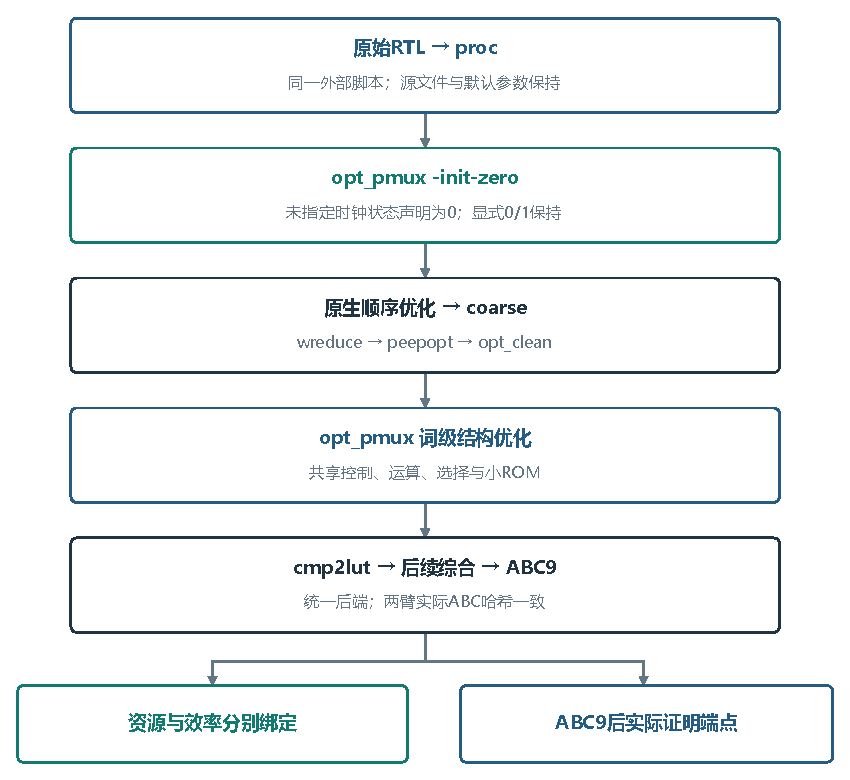
\includegraphics[width=14.4cm]{images/architecture.pdf}
\par\vspace{4pt}{\fontsize{10.5}{15.75}\selectfont 图1  源初态声明、PMUX重构及独立证据采集\par}
\end{minipage}\end{center}
最终Cyclone IV网表用于面积计数，ABC9后的ILANG用于可建模的形式端点。捕获端点必须与完整生产综合相对应，不能为了证明而改参数、换脚本或重新选择另一个候选。软件效率在完整综合运行中采集；形式证明与补充仿真独立执行，不混入综合耗时。

\Needspace{237.6pt}\subsubsection*{2.1.2  目标与版本选择}
设第i例原默认基线的LUT+NOT数为Bi，候选为Oi，九例基线均为正。每例不得增长且九例缩减率算术平均达到20\%，是同时检查的约束；总量加权结果只作补充。版本选择还须满足逐例效率与完整证明，不能仅凭更高面积均值替换已验证版本。

\[
R_i=\frac{B_i-O_i}{B_i}\times100\%,\quad i=1,\ldots,9
\]
\[
O_i\leq B_i,\qquad R_{\mathrm{mean}}=\frac{1}{9}\sum_{i=1}^{9}R_i\geq20\%
\]
结构准入与局部精确枚举不能构成最终LUT收益的全局最优性证明。保留零收益或小收益用例是约束下的实测选择，不表示该设计已达理论极限。性能门槛按每个用例分别判断，其他用例的加速不能抵消某例超过1.05的时间或内存比。

\Needspace{129.6pt}\subsubsection*{2.1.3  方法依据与职责边界}
Yosys提供词级优化和技术映射基础[3,4]，ABC为后端综合与验证提供实现[7]；决策图工作说明变量顺序和共享子图影响函数表示大小[8]。本项目用这些基础组织有界结构重写，再用实际映射与证明评价结果。文献中的节点数量或理论性质不能直接换算为本题得分。

\Needspace{222.5pt}
{\setstretch{1.0}\fontsize{10.5}{15.75}\selectfont
\begin{longtable}{>{\raggedright\arraybackslash}p{\dimexpr 0.204778\textwidth-2\tabcolsep\relax}>{\raggedright\arraybackslash}p{\dimexpr 0.382253\textwidth-2\tabcolsep\relax}>{\raggedright\arraybackslash}p{\dimexpr 0.412969\textwidth-2\tabcolsep\relax}}
\multicolumn{3}{c}{\normalsize 表3  各阶段的职责及不能推出的结论} \\[4pt]
\toprule
\bfseries 阶段 & \bfseries 职责 & \bfseries 限制 \\
\midrule
\endfirsthead
\multicolumn{3}{c}{\normalsize 表3  各阶段的职责及不能推出的结论（续）} \\[4pt]
\toprule
\bfseries 阶段 & \bfseries 职责 & \bfseries 限制 \\
\midrule
\endhead
\midrule\multicolumn{3}{r}{\small 续下页}\endfoot
\bottomrule\endlastfoot
源初态声明 & 为未指定时钟状态明确逻辑0，显式0/\allowbreak{}1不变 & 不是任意未知初态下的无条件等价变换 \\
词级重构 & 恢复控制关系并共享运算、选择与ROM余因子 & 局部结构改进不保证全部设计获益 \\
器件映射 & 统一Cyclone IV/\allowbreak{}ABC9后端形成面积端点 & 综合软件耗时不是器件关键路径 \\
完整EQY & 证明源逻辑初态契约下候选全部输出 & 不扩展为任意内部初态全集等价 \\
ModelSim & 观察初始化、复位、数据变化与结束计数 & 有限采样不替代形式证明或物理时序验证 \\
\end{longtable}
}
\Needspace{129.6pt}\subsection*{2.2  硬件系统介绍}
作品为综合软件，不包含自制硬件。Cyclone IV是统一映射目标；软件进程工作集并非FPGA片上RAM，综合墙钟并非电路时延。本书不报告未经布局布线的最高频率、功耗或实物资源收益。正式九例之外的规模测试必须单独保留输入与运行证据，不能混入九例均值。

工程在Windows原生环境运行。复现入口设置ABC与PATH，指向两臂共用的ABC二进制及所需运行库；本ABCEXTERNAL构建读取ABC环境变量。性能工具逐次解析实际ABC命令并校验文件哈希，确认比较中两臂确实使用同一后端。应通过提供的入口启动，不能把未配置依赖的裸EXE调用视为同一运行条件。

\Needspace{292.6pt}\subsection*{2.3  软件系统介绍}
\Needspace{237.6pt}\subsubsection*{2.3.1  初始化契约及其插入位置}
未指定初态、逻辑零初态和映射寄存器物理全零是三个不同概念。设逻辑状态q在映射中用反相信号r表示，q=\ensuremath{\neg}r，则q(0)=0要求r(0)=1。将两端物理寄存器都强制为0，会把这种合法编码误当成状态不一致；若先让优化器消去未初始化的常量历史寄存器，再补初值，也可能已经丢失初始行为。

\[
q=\neg r,\qquad q(0)=0\ \Longrightarrow\ r(0)=1
\]
实现因此在原synth\_\allowbreak{}intel的proc之后立即声明时钟FF的未指定初值。显式0与1逐位保持；未定义位写入init=0，声明本身不反相显式1。时钟极性、复位值、复位优先级和使能行为不由本阶段改写。后续原生优化在这些属性已明确后进行，从而把初始化语义带到实际器件端点。

初始化处理与一般逻辑化简严格区分：它选择一个源级初态契约，不声称对原本任意内部初态的设计保持全集行为。该约束不作用于自由输入，也不能把组合X、ROM无关项或不支持的锁存器都一律填成0。默认外部脚本不增加任何初始化命令，入口集成由候选二进制承担。

\Needspace{129.6pt}\subsubsection*{2.3.2  可写RAM、ROM与微例验证}
r11扩展在受支持的可写同步RAM上补充未知存储位，保留已有初始化数据、位掩码和地址偏移。有效写端口必须共享同一个信号时钟及极性；异步写、宽写、不同写时钟、已合并同步读端口等不支持结构明确报错。预算为每RAM最多16M位、设计累计存储及已有初始化扫描最多64M位、最多65536个新增初始化段。

没有有效运行时写端口的ROM保持不变，其X可能描述组合无关项，不是待补的存储初态。锁存器尚不在已验证范围内，不能列为通过。微例测试覆盖显式1、混合初值、使能、异步复位、常量历史及不同RAM初始化情况；r11共10例具备已检查的PASS证据，另有3例幂等检查。部分输出单独归纳未证出的UNKNOWN原记录保留，后续联合状态关系作为同一分区的待证输出，不能把它们直接当假设。

微例的候选侧只执行规定的存储展开与清理，不再追加zinit或setundef补零；这说明该初始化模块本身完成了声明。微例仅验证这一阶段，不自动证明后续完整默认综合流水。正式九例的完整证明、候选端点初始化审计和版本哈希另行记录，两类证据不能互相冒名。

\Needspace{129.6pt}\subsubsection*{2.3.3  精确控制恢复与词级共享}
选择器控制经常由少量输入译码而来。实现回溯至多6个控制位，对最多64种二态赋值逐项求值，要求每项为唯一有效分支或默认分支；多分支同时有效、函数不可识别或预算超限时保留原结构。输出位使用共享决策节点，常量直接连接，显式X/\allowbreak{}Z叶不被此规则任意补0或1。

\begin{center}\begin{minipage}{\textwidth}\centering
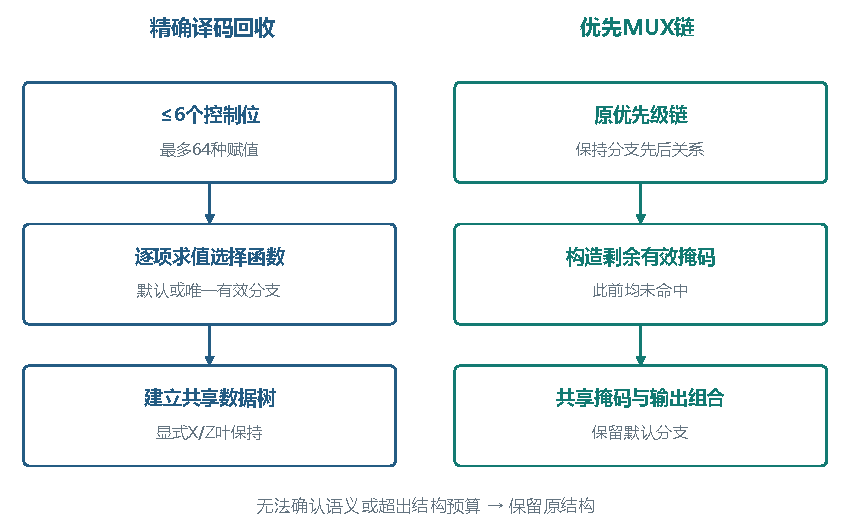
\includegraphics[width=14.4cm]{images/control_recovery.pdf}
\par\vspace{4pt}{\fontsize{10.5}{15.75}\selectfont 图2  小支持集控制恢复与保持优先级的掩码\par}
\end{minipage}\end{center}
\Needspace{8\baselineskip}
优先MUX链按既有先后顺序生成剩余有效掩码。第j个分支只能在自己的选择有效且此前均未命中时生效；默认分支对应全部未命中。这样可以共享控制而不把优先选择错误解释为独立one-hot输入。枚举证明限定在支持的控制逻辑内，不代表整个后端面积全局最小。

\[
m_j=s_j\land\bigwedge_{k<j}\neg s_k,\qquad m_{\mathrm{default}}=\bigwedge_k\neg s_k
\]
conev2跨多层选择整理控制和算术，banksv2共享双输出bank的行选择并保留例外分支，全字资源共享处理XOR、ADD、SUB。操作宽度、符号扩展和消费者必须保持；SUB左右操作数不能任意调换。公共运算提到选择之后会引入新的选择逻辑，因此仍需最终映射判断净收益。

\begin{center}\begin{minipage}{\textwidth}\centering
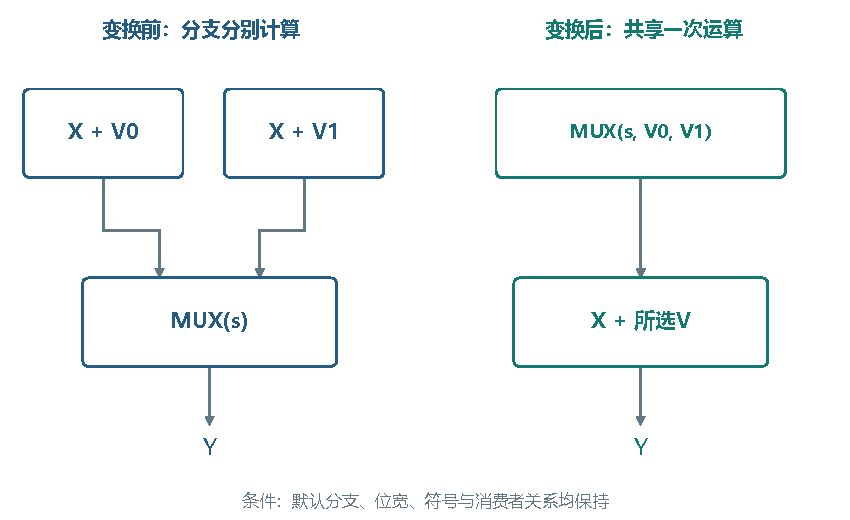
\includegraphics[width=14.4cm]{images/word_factor.pdf}
\par\vspace{4pt}{\fontsize{10.5}{15.75}\selectfont 图3  保持位宽与截断语义的公共加法提取\par}
\end{minipage}\end{center}
\[
\operatorname{mux}(s,X+V_0,X+V_1)=X+\operatorname{mux}(s,V_0,V_1)
\]
闭合选择DAG整理重用重复子图，闭合条件要求掌握所涉及节点的外部消费者，避免新结构生成后旧运算仍不得不保留。keep等保护属性、默认分支及外部使用关系都属于准入条件。词级共享和逐位布尔化简相互补充，不能把最终组合收益平均分配给每个模块而称为消融结果。

\Needspace{129.6pt}\subsubsection*{2.3.4  有界小ROM共享与候选顺序}
小ROM规则接受完整的5地址位、32字常量表，对2—16位输出建立精确余因子表示，一次最多处理8个符合条件的ROM。不同输出若拥有相同或互补的子函数，可复用节点；仅依赖剩余地址位的函数按支持集约简。它改变组合实现而不补写ROM数据，不改时钟或状态，也不调用外部映射器挑选结果。

规则以地址宽度、完整常量内容、输出宽度与保护属性限定应用范围，不能以test4名字识别机会。小ROM共享与初始化声明分别解决组合重复和状态契约问题，两者不能混为“把X填0以换面积”。保留真实映射结果，即使局部逻辑更紧凑也不预先宣称达到理论最优。

\Needspace{8\baselineskip}
精确ROM残差机制进一步利用各输出与简单函数之间的结构关系。对每个输出，从0、1、单个地址位及其反相中选取与完整真值表Hamming距离最小的基函数b；距离仅用于选择表达方式，不是允许的输出误差。随后对32个地址计算完整输出向量与基函数向量的逐位异或\ensuremath{\delta}，把\ensuremath{\delta}相同的地址划入集合G\ensuremath{\delta}。

\[
y_j=b_j\oplus\bigvee_{\delta_j=1}[x\in G_\delta]
\]
每个输出由基函数与相应地址集合的指示函数异或恢复，全部32个地址都必须逐项验证。残差描述的是精确修正项，绝不以较小Hamming距离替代功能正确。候选与原结构采用相同AIG结构估价：预计至少减少4个节点且减少比例至少1/\allowbreak{}8才准入；它只是有界候选筛选，不能保证ABC最终LUT也按同样比例下降。原ROM保护条件、完整常量要求和32地址校验保持，未满足条件时使用原余因子实现回退。

闭合DAG重构可能暴露原来分散的算术分支。后DAG阶段重新收集有界控制支持集，在最多256种赋值上证明互斥，才共享私有算术结果。前一阶段曾经观察到的互斥不能不经检查地沿用到重写后的图；对外仍有消费者的运算不能按私有结果删除。该规则是否属于当前候选由源码特征清单与版本绑定确认。

已确认的选择分支还为局部表达提供常量条件。当前候选将这些条件用于受限的分支常量传播，减少残留重复选择；传播后仍需维持完整控制真值与默认分支关系。该过程属于候选内部结构重构，不允许把当前仿真输入或某例已观察到的状态当作全局常量。

\Needspace{237.6pt}\subsubsection*{三位混合运算的共享进位／借位链}
该规则只接受WIDTH=3、S\_\allowbreak{}WIDTH=3的PMUX，三个完整分支恰为XOR、ADD和SUB各一个；通过真实译码证明选择互斥且三臂可达。每个算子的A\_\allowbreak{}SIGNED与B\_\allowbreak{}SIGNED必须同为合法0或1；不同算子可分别采用有符号或无符号解释，A/\allowbreak{}B/\allowbreak{}Y均严格为3位。以减法右操作数q为共同数，加法和异或可交换输入以对齐q。先根据选择信号选出另一操作数u，令s表示减法选择、a表示加法或减法选择，初始进位／借位c\ensuremath{{}_0}=0。三种结果共用下面的逐位关系：

\[
y_i=u_i\oplus q_i\oplus c_i
\]
\[
g_i=(u_i\oplus s)\land q_i,\qquad p_i=u_i\oplus s\oplus q_i
\]
\[
c_{i+1}=a\land(g_i\lor(p_i\land c_i))
\]
加法模式得到进位，减法模式得到借位，异或模式由a=0关闭传递。只生成第1、2位所需的传递项，末位输出之外的carry-out按原三位模8语义丢弃。实现保持原PMUX的A、S、Y和全部状态不变，将三个B分支接到同一共享结果；没有采用后来被拒绝的末级选择器折叠。

适用条件要求运算结果完整且私有，在根PMUX的A/\allowbreak{}B/\allowbreak{}S各端口中每位只使用一次；保护对象、冲突驱动、外部消费者、截片或扩宽均拒绝。签名参数不合法或同一算子的A/\allowbreak{}B签名不匹配时不应用该规则。最多检查64个候选根、改写16个，不外推到4位或任意位宽。结构重写的正确性仍由当前完整EQY和最终映射资源核验，不能用局部原型的更低门数替代原生程序结果。

r21把上述同宽模8关系扩展到合法匹配的signed参数。独立真实有符号源例在默认完整综合中由r20的18 LUT降为16 LUT，17位外部输入全部自由的原源到实测映射端点SAT证明通过，未使用符号范围或one-hot假设。这属于覆盖能力补充，未加入官方九例或均值，也不把r21的独立SAT记录改称当前候选新执行。

\Needspace{237.6pt}\subsubsection*{四分支零默认优先链的精确分组}
当前规则还识别恰好四层、字宽2—256位的MUX优先链，最终默认输入必须全部为已知0。按从高到低的原优先级，将前两分支组合为H、后两分支组合为L：H由s\ensuremath{{}_0}选择d\ensuremath{{}_0}或按s\ensuremath{{}_1}屏蔽的d\ensuremath{{}_1}，L由s\ensuremath{{}_2}选择d\ensuremath{{}_2}或按s\ensuremath{{}_3}屏蔽的d\ensuremath{{}_3}。只有前两选择均不成立时才开放低组，输出关系为：

\[
Y=H\lor((\neg s_0\land\neg s_1)\land L)
\]
该分组完整保留多选同时成立时的先后关系，不要求one-hot假设，也不把优先链改成无优先级的并联选择。所有内部链输出只允许一个消费者，连接必须连续且由对应MUX唯一驱动；保护对象、受保护别名、bank局部标记、输入驱动冲突、回馈至自身链输出及未知常量均拒绝。普通别名和重复选择信号仍合法。四臂零默认候选未通过保护检查时跳过该根；非四臂或非零默认继续原路径。

规则复用已有连线与消费者索引，不为每条四分支链重复建立完整结构上下文。当前test2面积收益由默认原生综合、完整源逻辑零证明及v3实测共同确认，未修改原源文件的敏感列表或在运行时固定输入。

r22引入的扫描跳过规则在当前候选中保留：全部前置helper之后统计模块内所有MUX，包含未被选择的内部单元；少于三个时不构造供priorities使用的只读Net，也不调用该步骤。原优先链规则至少需要三个不同MUX才能重写，因此这一条件下没有可触发根。后续PMUX控制恢复所用的第二个Net保留；这一步不改初始化、结构发射、标准pass或ABC。r22当时的官方九例面积与r20/\allowbreak{}r21相同；不同批次的墙钟差不能据此解释为该跳过条件带来的因果性能收益。

\Needspace{237.6pt}\subsubsection*{2.3.5  可观察状态保持与公共译码因子联合重写}
组合节点的每一时刻电平未必都被状态单元采样。该规则先检查PMUX完整输出Y的所有消费者：只允许未保护、使能高有效的DFFE，且D端完整同序连接Y，其他端口不再观察Y。再以该PMUX自身的等值码集合C构造active，而不是借用整个bank的选择信号。每个消费者的EN必须通过受限AND结构含有active这一必要因子；常量EN及未能证明的结构均跳过，不利用不可满足使能作为化简条件。

\[
\mathrm{EN}\Rightarrow\mathrm{active}=\bigvee_{k\in C}S_k,\qquad f_j(c)=d_j(c)\quad(\forall c\in C)
\]
\Needspace{8\baselineskip}
对每一输出位，从常量0、1、某一选择输入位及其取反中，选取在C内所有码字都与原所选数据相等的函数f。以任一受影响触发器为例，EN=0时两侧均保持当前Q；EN=1时必有一个有效码，原D与f在该码上相同。因此改写保持任意二值当前Q下的下一状态。原PMUX默认输入须全部为X，已知默认值或Z不进入该规则；结论是受使能约束的采样状态转移保持，不能写成未使能时D在全域四态下相等。

\[
Q^{\prime}=(\mathrm{EN}\ ?\ D:Q)=(\mathrm{EN}\ ?\ f:Q)
\]
\Needspace{8\baselineskip}
同一选择变量的完整等值译码还可能含有共同文字。令H比较所有码字共有的位，Rk比较剩余位，则每个原比较可精确分解为H与Rk。实现保留原比较对象、输出连线、属性及全部消费者；这一因式分解自身保持0/\allowbreak{}1/\allowbreak{}X/\allowbreak{}Z的比较语义。它与前述状态投影职责不同：只有完整译码组、用作识别起点且继续保留的PMUX，以及至少两个可投影PMUX共同通过检查后才一次提交，不单独开启care投影。

\[
\mathrm{eq}_k(x,c_k)=H(x_{\mathrm{common}},c_{\mathrm{common}})\land R_k(x_{\mathrm{remaining}},c_{k,\mathrm{remaining}})
\]
适用范围有明确边界：选择宽度5—8位，完整bank含3—8个互异、已知的无符号等值比较，共同位2—4位、剩余位1—4位，care输出1—16位且有2—8臂。每个计划逐项复核全部32—256种二值赋值，数量由选择位宽确定。输入锥只接受明确白名单并在主输入或有时钟状态Q处截断；未知、缺失或冲突驱动、循环、计划输出回流、额外观察者以及受保护对象均拒绝。扫描深度、节点数和提交次数亦受预算限制。

r23开发验证覆盖匿名重排总线、负文字投影和多个合法观察者：5个正例完成任意当前Q的采样下一状态SAT证明；17个拒绝例的完整JSON保持逐字节不变。公共因子另通过196608条四态等式检查，此检查不扩展为care投影的独立四态等价证明。这些记录用于检查通用守卫，未计入正式九例。

为检查组合效果，补充实验固定同一r21中间快照、工具、ABC和映射后缀；各次对照端点逐字节相同，正常脚本仅输入路径不同。表3a是开发期中间网表原型记录；正式r23将通用守卫与联合重写编入C++ pass，外部入口仍是同一read\_\allowbreak{}verilog和synth\_\allowbreak{}intel。

\Needspace{145.0pt}
{\setstretch{1.0}\fontsize{10.5}{15.75}\selectfont
\begin{longtable}{>{\raggedright\arraybackslash}p{\dimexpr 0.245734\textwidth-2\tabcolsep\relax}>{\raggedright\arraybackslash}p{\dimexpr 0.177474\textwidth-2\tabcolsep\relax}>{\raggedright\arraybackslash}p{\dimexpr 0.122867\textwidth-2\tabcolsep\relax}>{\raggedright\arraybackslash}p{\dimexpr 0.453925\textwidth-2\tabcolsep\relax}}
\multicolumn{4}{c}{\normalsize 表3a  同一冻结控制流下的四组原型结果} \\[4pt]
\toprule
\bfseries 配置 & \bfseries LUT+NOT & \bfseries DFF & \bfseries 证明记录 \\
\midrule
\endfirsthead
\multicolumn{4}{c}{\normalsize 表3a  同一冻结控制流下的四组原型结果（续）} \\[4pt]
\toprule
\bfseries 配置 & \bfseries LUT+NOT & \bfseries DFF & \bfseries 证明记录 \\
\midrule
\endhead
\midrule\multicolumn{4}{r}{\small 续下页}\endfoot
\bottomrule\endlastfoot
对照 & 12 & 14 & 本次未新增对照EQY \\
仅care投影 & 13 & 14 & 本次源逻辑0\ensuremath{\rightarrow}实际端点PASS \\
仅公共因子H & 12 & 14 & 既有完整PASS，重新核对端点 \\
care与H组合 & 9 & 14 & 既有完整PASS，重新核对端点 \\
\end{longtable}
}
四组映射结果的交互差值为9\ensuremath{-}13\ensuremath{-}12+12=-4，说明该固定流程下收益不可相加；它不定位ABC内部机理，也不保证其他设计获益。只有新增care候选在本次新跑完整证明，不能说四组都重新证明或它们属于正式九例。旧r18b快照的care-only 12\ensuremath{\rightarrow}13单列历史，不混入表3a。

当前正式test3的原默认面积基线为13，本候选为9个LUT+NOT，按完整原生综合、源逻辑零EQY和v3测量共同核验。原型的12个逻辑单元不是这份正式面积基线；实验也不消除C149.1答复的解释歧义。第3.3.1节的真实波形展示一个可核实输出位的保持与采样过程，有限记录不替代形式证明。

\Needspace{129.6pt}\subsubsection*{2.3.6  PMUX采样边界的同步复位与使能重述}
只整理组合数据树仍可能留下由保持行为形成的反馈选择。厂商指南指出，专用寄存器控制按异步清零、使能、同步清零、同步装载、数据的顺序生效；当RTL把同步复位放在使能之前时，综合可能用数据路径逻辑实现使能[10]。该说明提示表示方式会影响硬件控制端的利用，但并不保证某次Yosys改写必然节省LUT；本项目另以实际网表和完整证明核验。

\Needspace{8\baselineskip}
本规则只识别私有完整PMUX输出连接到正沿、正使能、正同步复位且复位值全0的\$sdffe。令R为原同步复位、E为原使能，D与Q分别为输入和当前状态，其上升沿转移为：

\[
Q^{\prime}=R\ ?\ 0:(E\ ?\ D:Q)
\]
\Needspace{8\baselineskip}
此重述阶段保持同一FF对象及D、Q、CLK、SRST、参数、属性和线网初值，只把类型重述为使能优先的\$sdffce，并令新使能E\ensuremath{^{\prime}}=E\ensuremath{\lor}R。新转移写为：

\[
E^{\prime}=E\lor R,\qquad Q^{\prime}=E^{\prime}\ ?\ (R\ ?\ 0:D):Q
\]
\Needspace{125.0pt}
{\setstretch{1.0}\fontsize{10.5}{15.75}\selectfont
\begin{longtable}{>{\raggedright\arraybackslash}p{\dimexpr 0.116041\textwidth-2\tabcolsep\relax}>{\raggedright\arraybackslash}p{\dimexpr 0.136519\textwidth-2\tabcolsep\relax}>{\raggedright\arraybackslash}p{\dimexpr 0.136519\textwidth-2\tabcolsep\relax}>{\raggedright\arraybackslash}p{\dimexpr 0.610922\textwidth-2\tabcolsep\relax}}
\multicolumn{4}{c}{\normalsize 表3b  任意二值D、Q下的控制分解} \\[4pt]
\toprule
\bfseries R & \bfseries E & \bfseries E\ensuremath{^{\prime}} & \bfseries 两种表示的下一状态 \\
\midrule
\endfirsthead
\multicolumn{4}{c}{\normalsize 表3b  任意二值D、Q下的控制分解（续）} \\[4pt]
\toprule
\bfseries R & \bfseries E & \bfseries E\ensuremath{^{\prime}} & \bfseries 两种表示的下一状态 \\
\midrule
\endhead
\midrule\multicolumn{4}{r}{\small 续下页}\endfoot
\bottomrule\endlastfoot
1 & 任意 & 1 & 0：复位不被外部使能屏蔽 \\
0 & 1 & 1 & D：正常采样 \\
0 & 0 & 0 & Q：保持当前状态 \\
\end{longtable}
}
R=1时新使能必为1，R=0时新使能等于原E，因此三行覆盖全部二值控制组合与任意当前Q、D。该规则不移动时钟边沿、不插入流水级，也不改变源初态契约；结论限于此同步状态转移，不宣称未知控制下的任意四态事件调度等价。标准kernel/\allowbreak{}ff.cc中的convert\_\allowbreak{}ce\_\allowbreak{}over\_\allowbreak{}srst已有同类控制恒等式；当前实现只在自定义pass的PMUX边界内选择结构，标准FF处理、dfflegalize和ABC均保持原样。

守卫逐项检查所有消费者，要求每个完整D端与PMUX.Y同序相连；其他读取端、公共Y输出、保护对象或别名、驱动冲突、缺失连接、非零或未知复位、负/\allowbreak{}非法极性及不支持FF均拒绝。Q可作为原有公开输出。宽度与PMUX臂数各限1—64，单根最多8个FF消费者；每模块最多保存64个候选、改写32个FF，整个设计最多检查128根、改写64个FF。全部只读计划完成后再提交，避免改写使已有消费者索引失效；相同控制对共享一个OR。

r28开发记录共36项：4个正例覆盖宽度1、3、64及两个完整FF消费者，对实际改写后网络进行任意前态Q、自由原输入的下一状态SAT证明；31个拒绝例与冻结r23输出JSON相同。另1项非法极性参数为2时未发生改写，进程以3221225725（0xC00000FD）退出，崩溃记录保留，不列为合法设计运行成功或完整等价通过。原对象、非EN端口、参数、属性和init另行逐项核对。

r28生产pipeline为450\ensuremath{\rightarrow}341个LUT+NOT，较r23的380再少39个，DFF仍为24。实际命中8个三位FF对象；其最终24个dffeas共用非恒定ENA，驱动LUT的四种控制赋值逐项满足ENA=en\ensuremath{\lor}rst。r28的SCLR仍接0，只能说明保持控制转到实际硬件使能端。后续目标专用映射与当期完整端点另行核验，不把旧开发记录改名为新运行，也不把单例减少量推广为普遍收益。

FAQ C34答复以最终网表效果评价其他优化方法[2]。本策略位于自定义pass的PMUX—FF采样边界，在分支常量传播之后、优先链与控制恢复之前执行；没有改动其他标准pass或依赖程序。该答复并未点名批准这一具体FF重述，C149.1的歧义仍保留。第3.3.1节仅用一个已核实对应输出位的真实有限波形解释保持与复位过程，整设计结论来自源逻辑零到实际端点的完整EQY。

\Needspace{237.6pt}\subsubsection*{2.3.7  Cyclone IV限定的硬件同步清零与初态编码}
前一阶段恢复硬件使能后，复位选择仍可能占用数据通路LUT。r29进一步在明确的Cyclone IV目标下连接寄存器SCLR端口。厂商控制优先级规定ENA先于同步清零[10]；因此保留新使能E\ensuremath{^{\prime}}=E\ensuremath{\lor}R，并将原复位R直接接入SCLR，得到：

\[
\mathrm{ENA}=E\lor R,\quad \mathrm{SCLR}=R,\quad Q^{\prime}=\mathrm{ENA}\ ?\ (\mathrm{SCLR}\ ?\ 0:D):Q
\]
R=1时ENA必为1，清零不会被外部E=0屏蔽；R=0时则恢复原使能采样或保持。此等式只给出二值控制域的状态转移依据，原生映射后的整设计正确性仍由实际端点完整EQY验证。

目标准入由synth\_\allowbreak{}intel的family=cycloneiv显式传入opt\_\allowbreak{}pmux -cycloneiv-sclr；其他器件族、不带此标志的命令及-init-zero模式不走这一映射。目标库还须提供端口方向、十个标量端口及两项参数均符合预期的dffeas黑盒声明。缺少目标声明或契约不合时保留通用\$sdffce路径，不因同名模块而启用。

映射继续使用私有完整PMUX—D边界、正极性和全0同步复位等守卫。提交前用FfInitVals读取实际逻辑Q初值：只接收每一位均已知0/\allowbreak{}1的完整FF字，冲突的已定义别名按输入错误处理；未知初值回退，不虚构0。每位初值分别编码为power\_\allowbreak{}up的low/\allowbreak{}high。只有已编码的Q位从线网init属性中清除，未改写位及其他Z位保留。

此目标映射将向量FF拆成等位数的标量dffeas，保留各位原CLK、D、Q与复位连接；它不再保留前一阶段的向量FF对象身份。先完成全部只读计划，再复用已生成的E\ensuremath{\lor}R、提交器件单元和初值属性修改，之后重建索引。没有增加后ABC重写步骤，也未修改标准映射pass或ABC。

\Needspace{128.0pt}
{\setstretch{1.0}\fontsize{10.5}{15.75}\selectfont
\begin{longtable}{>{\raggedright\arraybackslash}p{\dimexpr 0.150171\textwidth-2\tabcolsep\relax}>{\raggedright\arraybackslash}p{\dimexpr 0.525597\textwidth-2\tabcolsep\relax}>{\raggedright\arraybackslash}p{\dimexpr 0.324232\textwidth-2\tabcolsep\relax}}
\multicolumn{3}{c}{\normalsize 表3c  r29阶段独立模型的两个受限控制域} \\[4pt]
\toprule
\bfseries 域 & \bfseries 控制前提 & \bfseries 上升沿行为 \\
\midrule
\endfirsthead
\multicolumn{3}{c}{\normalsize 表3c  r29阶段独立模型的两个受限控制域（续）} \\[4pt]
\toprule
\bfseries 域 & \bfseries 控制前提 & \bfseries 上升沿行为 \\
\midrule
\endhead
\midrule\multicolumn{3}{r}{\small 续下页}\endfoot
\bottomrule\endlastfoot
沿用域 & SCLR=0；PRN=1；ASDATA/\allowbreak{}ALOAD/\allowbreak{}SLOAD=0；CLRN可为真实异步清零 & 保留原受限FF映射语义 \\
新增域 & CLRN=PRN=1；ASDATA/\allowbreak{}ALOAD/\allowbreak{}SLOAD=0；SCLR、ENA为二值控制 & ENA=0保持；否则SCLR=1清零；否则取D \\
\end{longtable}
}
两域均要求正沿时钟、真实时钟/\allowbreak{}Q连接和明确power\_\allowbreak{}up。新模型经过25项准入检查，以及任意前态、8个自由布尔输入的单步SAT和真实模型实现的时序归纳；后者包含两种显式初值，并核对旧域退化和形式/\allowbreak{}仿真模型一致性。r29资格批次的九例候选有58位处于新增SCLR域，其他位使用旧域；候选归一化不补zinit或setundef。模型不是通用厂商库，不证明未知控制的任意四态调度、异步与同步清零任意混合或器件延迟。首次小模型检查因缺运行库以0xC0000135启动失败，修正启动PATH后新批次通过；失败记录保留。

原生目标与初态检查另有5个映射正例、7个正常回退记录，其中4项与r28输出JSON逐字相同；1项冲突init按输入错误退出1。这些检查验证端口、初值和回退，不冒充独立语义证明。r29生产pipeline由原基线450降至323个LUT+NOT；r28为341，两者均24个FF。该单例差额和不同批次耗时不能直接推广为普遍收益或因果加速。

Cyclone IV手册说明每个LAB的同步清零是共享控制资源[11]。本项目核验逻辑资源数量与受限功能模型，没有完成布局布线、LAB控制共享可行性或板级时序验证。FAQ C34不是对这一具体器件映射的点名确认；C149.1的解释边界不因当前结果而消失。

\Needspace{129.6pt}\subsubsection*{2.3.8  互斥叶分支向同步装载端迁移}
r30在上一阶段的硬件同步清零基础上，把符合条件的一条PMUX数据分支交给SLOAD/\allowbreak{}ASDATA采样。规则仅作用于显式Cyclone IV目标，且原PMUX的所有完整D消费者已经通过私有边界、正沿时钟、正控制、全0同步复位和已知初态映射检查。真实译码逻辑必须证明三臂均可达且相互排斥，不能把独立选择输入假定为one-hot。

\Needspace{8\baselineskip}
三条B字中须恰有一条满足：字内各位均为直接主输入位，或来自单个时钟FF按原顺序排列的完整Q字。主输入位可来自不同端口，不要求覆盖整个端口；FF.Q截片、混合PI/\allowbreak{}Q、锁存器、重复数据位、不支持或冲突驱动及受保护对象均拒绝。全部D消费者都能完成目标转换后，才把选定B[j]接ASDATA、S[j]接SLOAD；任一消费者不合格，就不移除该臂。原PMUX的A、Y、属性和另两臂顺序保持，ENA=E\ensuremath{\lor}R、SCLR=R及CLK/\allowbreak{}Q/\allowbreak{}初态编码和状态位数不变。

\[
L=S_j,\quad A_s=B_j,\quad Q^{\prime}=\mathrm{ENA}\ ?(R\ ?\ 0:(L\ ?\ A_s:D_{\mathrm{rem}})):Q
\]
互斥条件下，L=1时原选择结果就是B[j]；L=0时剩余PMUX连同无选择默认A均与原结果相同。ENA=0保持Q；ENA=1时先判断同步清零，再判断同步装载，最后采样剩余D。因此选中装载但未使能时仍保持，同步清零也不会被装载遮蔽。D连接保留，但SLOAD=1时其组合值允许与旧D不同；保持的是二值采样状态转移，不是中间数据线全域相等。所有查询在提交前完成，后续控制恢复重建索引。

\Needspace{222.5pt}
{\setstretch{1.0}\fontsize{10.5}{15.75}\selectfont
\begin{longtable}{>{\raggedright\arraybackslash}p{\dimexpr 0.252560\textwidth-2\tabcolsep\relax}>{\raggedright\arraybackslash}p{\dimexpr 0.747440\textwidth-2\tabcolsep\relax}}
\multicolumn{2}{c}{\normalsize 表3d  当前受限模型的控制域与证据层次} \\[4pt]
\toprule
\bfseries 项目 & \bfseries 实际契约或结果 \\
\midrule
\endfirsthead
\multicolumn{2}{c}{\normalsize 表3d  当前受限模型的控制域与证据层次（续）} \\[4pt]
\toprule
\bfseries 项目 & \bfseries 实际契约或结果 \\
\midrule
\endhead
\midrule\multicolumn{2}{r}{\small 续下页}\endfoot
\bottomrule\endlastfoot
沿用域 & SCLR=ASDATA=SLOAD=0，PRN=1、ALOAD=0；CLRN可动态异步清零 \\
扩展域 & CLRN=PRN=1、ALOAD=0；ENA、SCLR、SLOAD、ASDATA、D可自由取二值；器件全局控制隐含正常1 \\
扩展域优先级 & 上升沿：ENA=0保持；否则SCLR清零；否则SLOAD取ASDATA；否则取D \\
模型独立检查 & 53项端口/\allowbreak{}参数边界；10自由布尔输入状态SAT；真实形式/\allowbreak{}仿真实现的时序归纳，含low/\allowbreak{}high初值 \\
实际厂商库观察 & 642次有限二值观察无差异；原总报告仍为ERROR，自动缓存刷新原因单列保存 \\
\end{longtable}
}
各实际端点必须先逐原语通过十标量端口、真实CLK/\allowbreak{}Q连线、无直接X/\allowbreak{}Z和明确power\_\allowbreak{}up等准入检查；显式器件全局端口不接受。候选证明侧不补zinit或setundef。扩展模型在SLOAD/\allowbreak{}ASDATA=0时退化为r29模型，并独立核对保持、清零优先、两种显式初值及形式/\allowbreak{}仿真实现一致性。它不是通用厂商库，不覆盖任意四态控制、活动器件全局复位、时序或亚稳态。首次模型检查因测试夹具中二进制字面量紧邻问号而解析失败；仅修正夹具空格，运行模型与runner未改，失败记录保留。

厂商指南给出ENA、同步清零、同步装载、数据的控制优先级[10]；本机既有Altera预编译库的独立探针进一步观察SLOAD选择ASDATA。已保存的321行、low/\allowbreak{}high两种初态共642次观察覆盖2种Q前态\ensuremath{\times}32种五位二值控制/\allowbreak{}数据组合，共64种元组，无行为差异。ModelSim自动刷新复制库的\_\allowbreak{}info并生成运行缓存，导致原报告的副本不可变检查为ERROR；原122个厂家库文件及原编译IR保持。这里引用有限行为观察，不将该ERROR改称整体PASS，也不称完成厂家模型形式证明。

随后另以本机Altera预编译DFFEAS库对R30九例完成一次有限功能复核，实际加载dffeas及PRIM\_\allowbreak{}GDFF\_\allowbreak{}LOW/\allowbreak{}HIGH，未编译自写DFFEAS。仅加入devclrn=devpor=1的正常器件工作条件，原十端口、power\_\allowbreak{}up/\allowbreak{}is\_\allowbreak{}wysiwyg及实际SCLR/\allowbreak{}SLOAD/\allowbreak{}ASDATA保持，未固定原RTL输入、复位或时钟。参考与候选合计643个FF实例的时间0 Q逐一一致，40684个有效采样无差异、X/\allowbreak{}Z或契约失败，CSV与冻结R30记录逐字节相同；643不是候选单侧的状态数。

该新批次与独立只读核验均通过。原厂家122文件、复制库原IR及全局ini不变，复制库自动生成的64位运行缓存单列审计；这不覆盖或改写先前探针的ERROR。LUT仍使用实际导出的真值表表达式，故结果仅称“使用真实厂家DFFEAS的九例有限功能复核”，不是完整厂商单元网表、SDF时序仿真或厂家形式证明。书中七张波形仍来自此前受限模型的新R30 VCD，不改称厂家库波形。

原生开发检查有7个正例，其中6项对任意当前状态和自由输入做下一步SAT；宽64另做完整元数据与端口检查。19项拒绝情况的完整JSON与r29逐字相同。首个证明夹具因线网和MUX使用同名标识而前端报错，修正夹具后重跑，候选源码和程序未重编；原错误保留。完整九例源到实际候选EQY是另一层证据。

正式pipeline为450\ensuremath{\rightarrow}305个LUT+NOT，FF仍24；r29为323。开发记录中八个外层PMUX各迁移一臂，四个主输入叶、四个完整时钟Q叶，最终24个SLOAD脚均非恒定。独立规模wrapper相对r29只从598降到593个逻辑单元，不能把单例减少18直接外推。硬件同步控制属于LAB共享资源[11]，尚未验证布局布线或共享控制的物理适配；C34和C149.1的解释边界仍保留。

\begin{center}\begin{minipage}{\textwidth}\centering
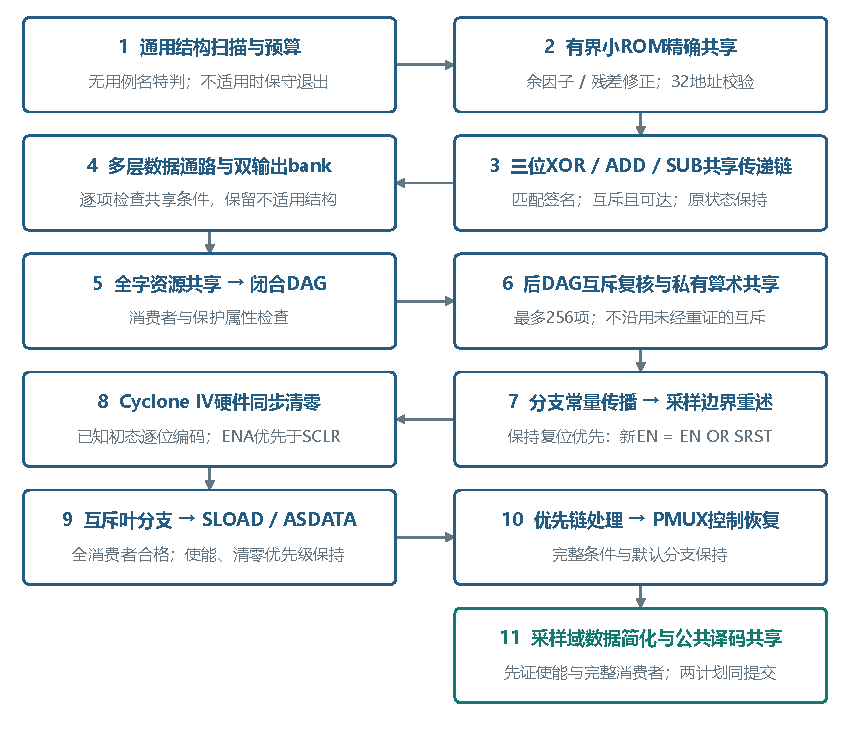
\includegraphics[width=14.4cm]{images/candidate_flow.pdf}
\par\vspace{4pt}{\fontsize{10.5}{15.75}\selectfont 图4  当前候选的通用结构处理及保守退出\par}
\end{minipage}\end{center}
\Needspace{129.6pt}\subsubsection*{2.3.9  源码及外部接口}
\Needspace{5\baselineskip}
{\small
\noindent\begin{minipage}{\linewidth}
\begin{verbatim}
read_verilog CASE.v
synth_intel -family cycloneiv -top TOP
\end{verbatim}
\end{minipage}
\par}
\texttt{CASE.\allowbreak{}v}与TOP来自固定九例清单；两臂使用相同脚本文件，差异仅在被调用的Yosys二进制。计时脚本仅含上述两条命令；全部计时结束后另行运行同样两条命令并附write\_\allowbreak{}json捕获资源网表，导出进程不进入效率统计。不修改WIDTH、LANES等默认参数。启动脚本设置同一ABC绝对路径并保留实际调用记录；脚本层面没有按用例选择某个内部算法的开关。

\Needspace{382.5pt}
{\setstretch{1.0}\fontsize{10.5}{15.75}\selectfont
\begin{longtable}{>{\raggedright\arraybackslash}p{\dimexpr 0.423208\textwidth-2\tabcolsep\relax}>{\raggedright\arraybackslash}p{\dimexpr 0.576792\textwidth-2\tabcolsep\relax}}
\multicolumn{2}{c}{\normalsize 表4  当前主要源码与职责} \\[4pt]
\toprule
\bfseries 文件 & \bfseries 职责 \\
\midrule
\endfirsthead
\multicolumn{2}{c}{\normalsize 表4  当前主要源码与职责（续）} \\[4pt]
\toprule
\bfseries 文件 & \bfseries 职责 \\
\midrule
\endhead
\midrule\multicolumn{2}{r}{\small 续下页}\endfoot
\bottomrule\endlastfoot
opt\_\allowbreak{}pmux.cc & 两个模式的注册、结构过滤与统一调度 \\
pmux\_\allowbreak{}init\_\allowbreak{}zero.h & 时钟FF及受支持可写RAM的源初态声明 \\
pmux\_\allowbreak{}share\_\allowbreak{}cone.h /\allowbreak{} pmux\_\allowbreak{}share\_\allowbreak{}banks\_\allowbreak{}v2.h & 多层数据通路、双输出bank及例外融合 \\
pmux\_\allowbreak{}resource\_\allowbreak{}share.h /\allowbreak{} pmux\_\allowbreak{}share\_\allowbreak{}dag.h & 全字运算共享、闭合选择DAG整理 \\
pmux\_\allowbreak{}small\_\allowbreak{}rom.h & 有界5位地址常量ROM共享及精确残差修正 \\
pmux\_\allowbreak{}rom\_\allowbreak{}residual.h & 基函数选择、残差地址组与全32地址精确校验 \\
pmux\_\allowbreak{}share\_\allowbreak{}carry3.h & 三位XOR/\allowbreak{}ADD/\allowbreak{}SUB共享传递链；支持同一算子A/\allowbreak{}B匹配的合法signed参数 \\
pmux\_\allowbreak{}priority\_\allowbreak{}grouping.h & 四分支、零默认优先链精确分组；不要求one-hot \\
pmux\_\allowbreak{}observable\_\allowbreak{}decode.h & 使能约束下的状态投影与公共译码因子联合提交 \\
pmux\_\allowbreak{}sdffe\_\allowbreak{}boundary.h & PMUX私有采样边界复位/\allowbreak{}使能重述；保持状态转移 \\
pmux\_\allowbreak{}cycloneiv\_\allowbreak{}sload.h & 三臂互斥PMUX完整叶分支向SLOAD/\allowbreak{}ASDATA迁移 \\
pmux\_\allowbreak{}cycloneiv\_\allowbreak{}sclr.h & 显式Cyclone IV目标的SCLR映射及已知初态逐位编码 \\
synth\_\allowbreak{}intel.cc /\allowbreak{} CMakeLists.txt & proc后与coarse的固定调用；编译进主程序 \\
\end{longtable}
}
\Needspace{129.6pt}\subsubsection*{2.3.10  完整形式证明与旧反例的关系}
本轮主证明从原RTL的逻辑零初态契约直接到当前候选的实际默认综合端点。gold侧将未指定时钟FF初态明确为0并保持显式初值；gate侧读取捕获的实际ABC9后端点，再以受限dffeas模型解释映射power\_\allowbreak{}up和控制。源RTL、参数、候选二进制、生产端点及证明副本均以哈希关联。

\begin{center}\begin{minipage}{\textwidth}\centering
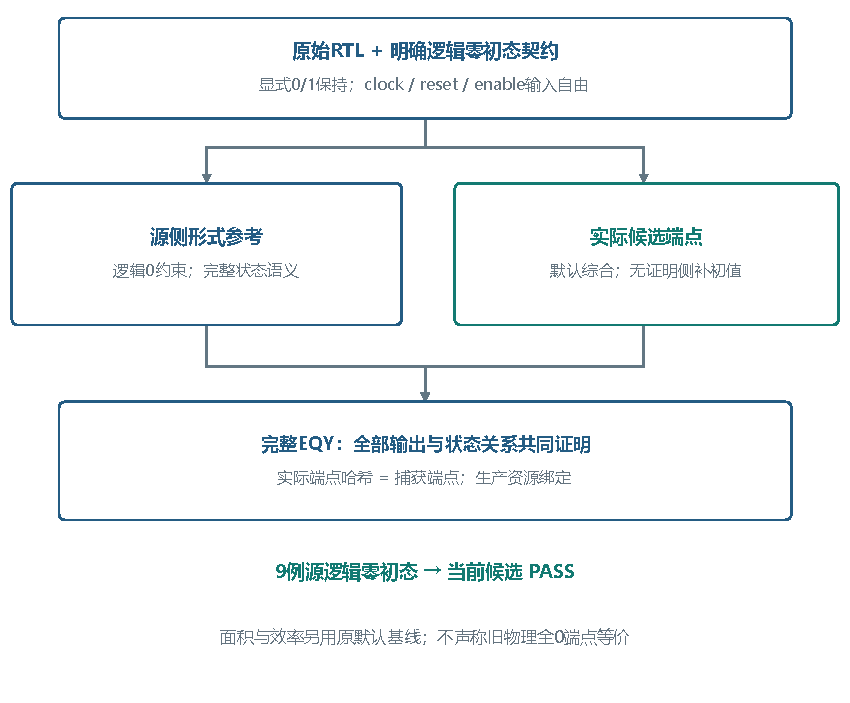
\includegraphics[width=14.4cm]{images/proof_chain.pdf}
\par\vspace{4pt}{\fontsize{10.5}{15.75}\selectfont 图5  源逻辑初态契约到实际候选的证明与证据绑定\par}
\end{minipage}\end{center}
完整证明保留自由外部输入；clock、reset、enable不被固定成有利激励。clk2fflogic保留实际输入时钟边沿关系，全部顶层输出及所需状态关系置于同一分区共同证明基础情况和归纳步骤。内部匹配状态不作为未经证明的切点假设。工具报告内历史字段名baseline在此运行中指向送入runner的候选，必须按端点哈希解释角色，不能据名称误报为原默认基线。

当前候选证明侧不追加zinit或setundef初始化修补；受限逆映射读取端点实际power\_\allowbreak{}up属性，初始化结论由实际综合产物承担。源侧零初始化与候选侧归一化承担不同职责，完整脚本和初始化审计随证明记录保留。

端点初始化检查共覆盖320个状态位，逆映射后的显式0为319位、显式1为1位，未知位为0；每个映射dffeas均实际携带power\_\allowbreak{}up高或低参数，不借用模型默认值补齐。这里的init属性来源是当前候选的实际映射参数，不能说成用户原RTL本来就写有这些初始化声明。

r09旧链保留原RTL的未指定初态，按EQY未知值语义证明定义行为精化，再比较同映射初态端点。它并未证明源逻辑全0时的初始输出。新方法对“逻辑零初态”这一具体要求给出更直接的保证：初始行为在实际综合前被约束，并从源直接证明到交付候选；这不等同于声称新证明在任意初态关系上都是旧证明的超集。

旧默认基线的test4严格逻辑零反例仍真实存在。源逻辑0与旧映射物理0的反相编码不一致，不会因新程序通过而消失。因此必须区分两项成立的陈述：面积对照仍使用原默认基线；功能证明使用源逻辑零契约及新候选。不能同时要求旧基线物理0与新候选物理0直接等价，并声称它们都代表源逻辑0。

\Needspace{184.6pt}\section*{第三部分  完成情况及性能测试}
\Needspace{129.6pt}\subsection*{3.1  完成情况}
以下结果仅对应r30\_\allowbreak{}native\_\allowbreak{}sload及本次绑定文件[9]。原4例和新增5例保持源文件字节与默认参数，未将扩展研发样本加入正式均值。版本、工具哈希、原始测量、每例证明端点和报告SHA-256保存于证据清单。

本轮九例各自均超过20\%，最低为test4的22.2222\%。这是当前默认用例的逐项实测；FAQ规定的正式聚合口径仍是九例缩减率等权平均。

\Needspace{256.5pt}
{\setstretch{1.0}\fontsize{10.5}{15.75}\selectfont
\begin{longtable}{>{\raggedright\arraybackslash}p{\dimexpr 0.204778\textwidth-2\tabcolsep\relax}>{\raggedright\arraybackslash}p{\dimexpr 0.423208\textwidth-2\tabcolsep\relax}>{\raggedright\arraybackslash}p{\dimexpr 0.372014\textwidth-2\tabcolsep\relax}}
\multicolumn{3}{c}{\normalsize 表5  正式九例及结构范围} \\[4pt]
\toprule
\bfseries 用例 & \bfseries 结构摘要 & \bfseries 状态特征 \\
\midrule
\endfirsthead
\multicolumn{3}{c}{\normalsize 表5  正式九例及结构范围（续）} \\[4pt]
\toprule
\bfseries 用例 & \bfseries 结构摘要 & \bfseries 状态特征 \\
\midrule
\endhead
\midrule\multicolumn{3}{r}{\small 续下页}\endfoot
\bottomrule\endlastfoot
test1 & 16状态寄存数据选择 & 异步高有效复位 \\
test2 & 组合优先选择 & clk未使用；原敏感列表保持 \\
test3 & 移位寄存器与GPIO更新 & 无显式初始化/\allowbreak{}复位 \\
test4 & 5b到6b寄存译码 & 异步低有效复位；部分状态复位未赋值 \\
balanced & 平衡数据选择结构 & 按源文件默认配置 \\
pipeline & 流水数据通路 & 按源文件默认配置 \\
crossbar & 交叉选择结构 & 按源文件默认配置 \\
feedback & 反馈数据通路 & 按源文件默认配置 \\
nested & 嵌套选择结构 & 按源文件默认配置 \\
\end{longtable}
}
test2原RTL敏感列表会影响事件驱动仿真的触发方式。源到候选EQY采用Yosys read\_\allowbreak{}verilog/\allowbreak{}proc的综合解释；ModelSim比较的是映射参考与实际候选，不能据此声称已复现原RTL事件敏感列表的逐事件行为。形式和仿真各自说明输入、端点与初态，不利用修订源文件或缩小参数把面积、证明和波形混成同一项证据。

\Needspace{184.6pt}\subsection*{3.2  工程成果}
\Needspace{129.6pt}\subsubsection*{3.2.1  冻结工具与测量政策}
基线来自公开提交d0e71cfb7bcafe2b437f3edc1789b69e99ecd55a；候选包含内置pass及固定集成调用。官方FAQ提及的dirty补丁未公开，本地可复现对照不等于已认证官方未公开二进制。两臂使用同一ABC文件，逐次实际命令与SHA-256检查结果写入测量报告；不能由日志中的占位显示名称反推它忽略了ABC环境设置。

当前采用v3 两命令生命周期。计时脚本仅含read\_\allowbreak{}verilog与synth\_\allowbreak{}intel；面积在全部计时结束后独立导出，并逐类型核对每次内置统计。这是C145展示命令范围的实现；C92未明确禁止导出，不能据此否定旧v2记录。

C145展示读取源文件与synth\_\allowbreak{}intel流程，C87/\allowbreak{}C92要求从Yosys启动至结束的全生命周期；本轮按展示命令确定进程内容。synth\_\allowbreak{}intel内置的统计、检查、日志以及等待ABC仍计入时间，没有在综合内部扣除某段耗时。全部初测及复测结束后才开始独立面积捕获，源文件、工具、ABC、门库和脚本散列一并核对。

独立捕获的JSON用于按叶实例分类LUT、标量取反及DFF；每臂均与全部计时记录及首例基线预热的内置最终top统计逐类型核对。该关系证明资源清单一致，不等于计时进程曾输出JSON，也不证明两次网表逐位相同。完整网表与候选生产端点的绑定、EQY仍各自单独验证。

旧v2包含附加stat与JSON导出，历史成功和失败均按原范围保留。C92没有明确答复所有流程是否必须排除导出，因此本书不将v2称为无效数据；也不把v2与v3的时间差归因于算法改进。不同范围的结果不拼接为同一份通过报告。

计时为Yosys主进程创建到退出的墙钟，覆盖完整综合与等待ABC的流程；峰值工作集来自同一次运行的主进程PeakWorkingSetSize。EQY和ModelSim不在综合效率计时内。正式政策先对首例基线预热10次；初测若时间比或内存比超过1.05且符合短例条件，就完整复测五对，分别取两臂算术均值，初测不加入复测均值。全部记录保留，不提前停止或挑选最快样本。

主批r30\_\allowbreak{}run01因已记录的C盘空间事件，原基线安装在C盘、优化安装在D盘；原输入和公共ABC在C盘，计时输出及子进程TEMP/\allowbreak{}TMP在D盘，未修改系统环境。各比值严格采用该批次自身两臂记录。随后实际迁移All将两侧程序和输入置于同一D盘，作为独立复现，不能混合两批样本、挑选较优值或把存储环境差异解释为算法收益。

\Needspace{8\baselineskip}
本次九例均未触发复测，每例采用初始一对；这仍是一轮固定政策下的机器测量，不代表跨硬件及任意后台负载的统计保证。

\[
\frac{t_{\mathrm{opt}}}{t_{\mathrm{base}}}\leq1.05,\qquad\frac{M_{\mathrm{opt}}}{M_{\mathrm{base}}}\leq1.05
\]
\Needspace{305.0pt}\subsubsection*{3.2.2  逐例面积与算术平均}
{\setstretch{1.0}\fontsize{10.5}{15.75}\selectfont
\begin{longtable}{>{\raggedright\arraybackslash}p{\dimexpr 0.266212\textwidth-2\tabcolsep\relax}>{\raggedright\arraybackslash}p{\dimexpr 0.235495\textwidth-2\tabcolsep\relax}>{\raggedright\arraybackslash}p{\dimexpr 0.235495\textwidth-2\tabcolsep\relax}>{\raggedright\arraybackslash}p{\dimexpr 0.262799\textwidth-2\tabcolsep\relax}}
\multicolumn{4}{c}{\normalsize 表6  逐例LUT+NOT与缩减率（独立捕获）} \\[4pt]
\toprule
\bfseries 用例 & \bfseries 原默认基线 & \bfseries 当前候选 & \bfseries 缩减率 \\
\midrule
\endfirsthead
\multicolumn{4}{c}{\normalsize 表6  逐例LUT+NOT与缩减率（独立捕获）（续）} \\[4pt]
\toprule
\bfseries 用例 & \bfseries 原默认基线 & \bfseries 当前候选 & \bfseries 缩减率 \\
\midrule
\endhead
\midrule\multicolumn{4}{r}{\small 续下页}\endfoot
\bottomrule\endlastfoot
test1 & 288 & 204 & 29.1667\% \\
test2 & 25 & 15 & 40.0000\% \\
test3 & 13 & 9 & 30.7692\% \\
test4 & 36 & 28 & 22.2222\% \\
balanced & 426 & 239 & 43.8967\% \\
pipeline & 450 & 305 & 32.2222\% \\
crossbar & 408 & 241 & 40.9314\% \\
feedback & 368 & 208 & 43.4783\% \\
nested & 413 & 233 & 43.5835\% \\
总量／算术均值 & 2427 & 1482 & 36.2522\% \\
\end{longtable}
}
最后一行的前两项为单元总量，末项为九个逐例缩减率的等权算术平均36.2522\%。按总量计算的加权缩减38.9370\%另列，不用它代替评分均值。9/\allowbreak{}9例单独达到20\%；各例原始结果完整保留。

\begin{center}\begin{minipage}{\textwidth}\centering
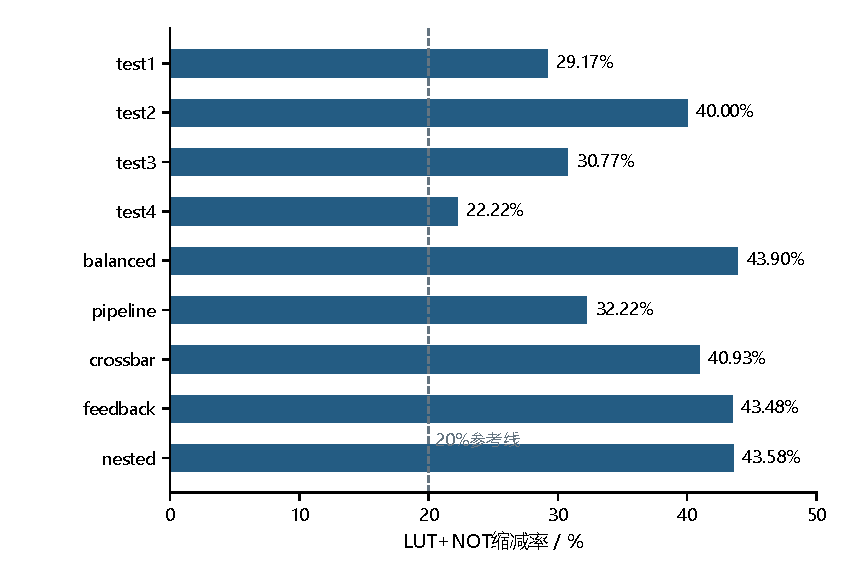
\includegraphics[width=14.4cm]{images/area_results.pdf}
\par\vspace{4pt}{\fontsize{10.5}{15.75}\selectfont 图6  九例缩减率；20\%虚线仅作参考，不是单例门槛\par}
\end{minipage}\end{center}
\Needspace{245.0pt}
{\setstretch{1.0}\fontsize{10.5}{15.75}\selectfont
\begin{longtable}{>{\raggedright\arraybackslash}p{\dimexpr 0.266212\textwidth-2\tabcolsep\relax}>{\raggedright\arraybackslash}p{\dimexpr 0.245734\textwidth-2\tabcolsep\relax}>{\raggedright\arraybackslash}p{\dimexpr 0.245734\textwidth-2\tabcolsep\relax}>{\raggedright\arraybackslash}p{\dimexpr 0.242321\textwidth-2\tabcolsep\relax}}
\multicolumn{4}{c}{\normalsize 表7  面积分类及状态单元核对} \\[4pt]
\toprule
\bfseries 用例 & \bfseries DFF 基线\ensuremath{\rightarrow}候选 & \bfseries LUT 基线\ensuremath{\rightarrow}候选 & \bfseries NOT 基线\ensuremath{\rightarrow}候选 \\
\midrule
\endfirsthead
\multicolumn{4}{c}{\normalsize 表7  面积分类及状态单元核对（续）} \\[4pt]
\toprule
\bfseries 用例 & \bfseries DFF 基线\ensuremath{\rightarrow}候选 & \bfseries LUT 基线\ensuremath{\rightarrow}候选 & \bfseries NOT 基线\ensuremath{\rightarrow}候选 \\
\midrule
\endhead
\midrule\multicolumn{4}{r}{\small 续下页}\endfoot
\bottomrule\endlastfoot
test1 & 222\ensuremath{\rightarrow}222 & 286\ensuremath{\rightarrow}202 & 2\ensuremath{\rightarrow}2 \\
test2 & 0\ensuremath{\rightarrow}0 & 25\ensuremath{\rightarrow}15 & 0\ensuremath{\rightarrow}0 \\
test3 & 17\ensuremath{\rightarrow}14 & 12\ensuremath{\rightarrow}8 & 1\ensuremath{\rightarrow}1 \\
test4 & 10\ensuremath{\rightarrow}10 & 35\ensuremath{\rightarrow}27 & 1\ensuremath{\rightarrow}1 \\
balanced & 12\ensuremath{\rightarrow}12 & 426\ensuremath{\rightarrow}239 & 0\ensuremath{\rightarrow}0 \\
pipeline & 24\ensuremath{\rightarrow}24 & 450\ensuremath{\rightarrow}305 & 0\ensuremath{\rightarrow}0 \\
crossbar & 10\ensuremath{\rightarrow}10 & 408\ensuremath{\rightarrow}241 & 0\ensuremath{\rightarrow}0 \\
feedback & 16\ensuremath{\rightarrow}16 & 367\ensuremath{\rightarrow}207 & 1\ensuremath{\rightarrow}1 \\
nested & 12\ensuremath{\rightarrow}12 & 413\ensuremath{\rightarrow}233 & 0\ensuremath{\rightarrow}0 \\
\end{longtable}
}
表7将触发器和逻辑单元分开报告，DFF变化不能混入LUT+NOT缩减率。源逻辑初态明确后可能影响状态优化结果，因此资源分类和功能证明必须绑定同一候选，不能从旧版本只拷贝更低的单元数。最终叶单元、I/\allowbreak{}O、unknown类别和默认参数原始统计均保留。

\Needspace{285.0pt}\subsubsection*{3.2.3  逐例效率与复测依据}
{\setstretch{1.0}\fontsize{10.5}{15.75}\selectfont
\begin{longtable}{>{\raggedright\arraybackslash}p{\dimexpr 0.204778\textwidth-2\tabcolsep\relax}>{\raggedright\arraybackslash}p{\dimexpr 0.218430\textwidth-2\tabcolsep\relax}>{\raggedright\arraybackslash}p{\dimexpr 0.218430\textwidth-2\tabcolsep\relax}>{\raggedright\arraybackslash}p{\dimexpr 0.204778\textwidth-2\tabcolsep\relax}>{\raggedright\arraybackslash}p{\dimexpr 0.153584\textwidth-2\tabcolsep\relax}}
\multicolumn{5}{c}{\normalsize 表8  v3 两命令：墙钟、比例及采用对数} \\[4pt]
\toprule
\bfseries 用例 & \bfseries 基线/\allowbreak{}s & \bfseries 候选/\allowbreak{}s & \bfseries 时间比 & \bfseries 对数 \\
\midrule
\endfirsthead
\multicolumn{5}{c}{\normalsize 表8  v3 两命令：墙钟、比例及采用对数（续）} \\[4pt]
\toprule
\bfseries 用例 & \bfseries 基线/\allowbreak{}s & \bfseries 候选/\allowbreak{}s & \bfseries 时间比 & \bfseries 对数 \\
\midrule
\endhead
\midrule\multicolumn{5}{r}{\small 续下页}\endfoot
\bottomrule\endlastfoot
test1 & 0.354915 & 0.314579 & 0.8864 & 1 \\
test2 & 0.183127 & 0.186038 & 1.0159 & 1 \\
test3 & 0.194104 & 0.193565 & 0.9972 & 1 \\
test4 & 0.220463 & 0.203602 & 0.9235 & 1 \\
balanced & 0.420389 & 0.312497 & 0.7434 & 1 \\
pipeline & 0.455909 & 0.412249 & 0.9042 & 1 \\
crossbar & 0.430290 & 0.310951 & 0.7227 & 1 \\
feedback & 0.389284 & 0.343896 & 0.8834 & 1 \\
nested & 0.403255 & 0.321552 & 0.7974 & 1 \\
\end{longtable}
}
\Needspace{245.0pt}
{\setstretch{1.0}\fontsize{10.5}{15.75}\selectfont
\begin{longtable}{>{\raggedright\arraybackslash}p{\dimexpr 0.259386\textwidth-2\tabcolsep\relax}>{\raggedright\arraybackslash}p{\dimexpr 0.259386\textwidth-2\tabcolsep\relax}>{\raggedright\arraybackslash}p{\dimexpr 0.259386\textwidth-2\tabcolsep\relax}>{\raggedright\arraybackslash}p{\dimexpr 0.221843\textwidth-2\tabcolsep\relax}}
\multicolumn{4}{c}{\normalsize 表9  v3 两命令：主进程峰值工作集及比例} \\[4pt]
\toprule
\bfseries 用例 & \bfseries 基线/\allowbreak{}字节 & \bfseries 候选/\allowbreak{}字节 & \bfseries 内存比 \\
\midrule
\endfirsthead
\multicolumn{4}{c}{\normalsize 表9  v3 两命令：主进程峰值工作集及比例（续）} \\[4pt]
\toprule
\bfseries 用例 & \bfseries 基线/\allowbreak{}字节 & \bfseries 候选/\allowbreak{}字节 & \bfseries 内存比 \\
\midrule
\endhead
\midrule\multicolumn{4}{r}{\small 续下页}\endfoot
\bottomrule\endlastfoot
test1 & 21544960.0 & 20643840.0 & 0.9582 \\
test2 & 14614528.0 & 14544896.0 & 0.9952 \\
test3 & 15474688.0 & 15421440.0 & 0.9966 \\
test4 & 16719872.0 & 16216064.0 & 0.9699 \\
balanced & 23568384.0 & 19464192.0 & 0.8259 \\
pipeline & 24395776.0 & 22245376.0 & 0.9119 \\
crossbar & 23375872.0 & 20172800.0 & 0.8630 \\
feedback & 22528000.0 & 20156416.0 & 0.8947 \\
nested & 23392256.0 & 20951040.0 & 0.8956 \\
\end{longtable}
}
最大时间比1.015894，最大内存比0.996559；两项逐例均不超过1.05。采用五对均值时，平均峰值字节可能出现小数，它是进程峰值计数的算术平均，不是单次计数精度改变。候选最长墙钟0.412249秒、最大峰值工作集22245376字节。

\begin{center}\begin{minipage}{\textwidth}\centering
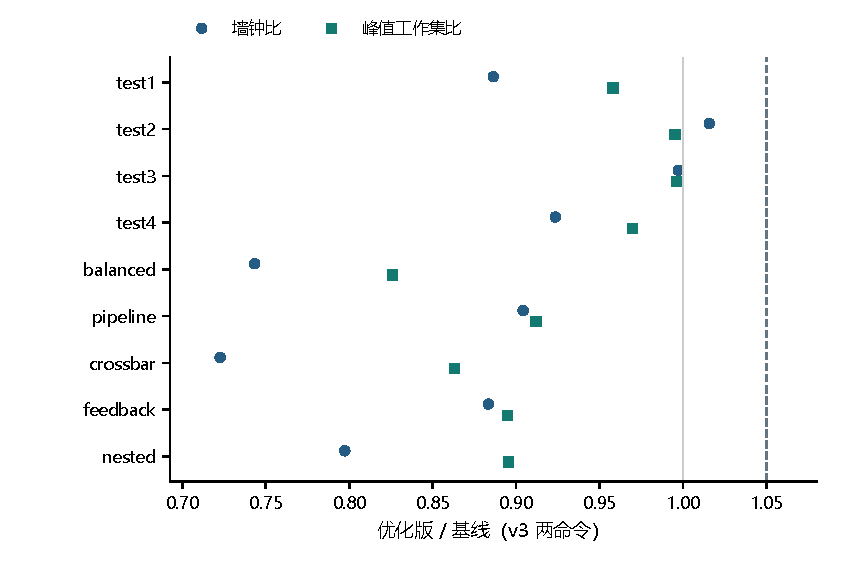
\includegraphics[width=14.4cm]{images/performance_results.pdf}
\par\vspace{4pt}{\fontsize{10.5}{15.75}\selectfont 图7  v3 两命令时间与工作集比；初测或五对复测按规则采用\par}
\end{minipage}\end{center}
面积下降与软件内存下降没有必然对应关系，局部重构也可能因扫描和构图增加运行时间。本项目把超过门槛的候选排除在当前最佳之外，保留其原始复测记录；不把更高均值包装成已达全部约束。当前近千节点证据另见补充规模段，独立于正式九例。

\Needspace{265.0pt}\subsubsection*{3.2.4  版本决策与完整证明}
{\setstretch{1.0}\fontsize{10.5}{15.75}\selectfont
\begin{longtable}{>{\raggedright\arraybackslash}p{\dimexpr 0.163823\textwidth-2\tabcolsep\relax}>{\raggedright\arraybackslash}p{\dimexpr 0.252560\textwidth-2\tabcolsep\relax}>{\raggedright\arraybackslash}p{\dimexpr 0.583618\textwidth-2\tabcolsep\relax}}
\multicolumn{3}{c}{\normalsize 表10a  含导出范围的研发记录（早期及v2）} \\[4pt]
\toprule
\bfseries 版本 & \bfseries 九例算术均值 & \bfseries 证据与范围内结论 \\
\midrule
\endfirsthead
\multicolumn{3}{c}{\normalsize 表10a  含导出范围的研发记录（早期及v2）（续）} \\[4pt]
\toprule
\bfseries 版本 & \bfseries 九例算术均值 & \bfseries 证据与范围内结论 \\
\midrule
\endhead
\midrule\multicolumn{3}{r}{\small 续下页}\endfoot
\bottomrule\endlastfoot
r09 & 24.0868\% & 早期含导出；定义行为精化，未证明源逻辑零初态 \\
r10 & 24.0621\% & 严格源初态证明；本范围效率通过 \\
r12 & 24.6794\% & 严格源初态证明；本范围效率通过 \\
r13 & 27.6987\% & 严格源初态证明；本范围效率失败 \\
r14 & 28.5534\% & 严格源初态证明；本范围效率失败 \\
r15 & 28.5534\% & 严格源初态证明；本范围效率通过 \\
r16 & 30.4053\% & 严格源初态证明；本范围效率失败 \\
r17 & 30.4053\% & 严格源初态证明；本范围效率失败 \\
\end{longtable}
}
\Needspace{245.0pt}
{\setstretch{1.0}\fontsize{10.5}{15.75}\selectfont
\begin{longtable}{>{\raggedright\arraybackslash}p{\dimexpr 0.163823\textwidth-2\tabcolsep\relax}>{\raggedright\arraybackslash}p{\dimexpr 0.252560\textwidth-2\tabcolsep\relax}>{\raggedright\arraybackslash}p{\dimexpr 0.583618\textwidth-2\tabcolsep\relax}}
\multicolumn{3}{c}{\normalsize 表10b  v3两命令范围的研发记录} \\[4pt]
\toprule
\bfseries 版本 & \bfseries 九例算术均值 & \bfseries 证据与范围内结论 \\
\midrule
\endfirsthead
\multicolumn{3}{c}{\normalsize 表10b  v3两命令范围的研发记录（续）} \\[4pt]
\toprule
\bfseries 版本 & \bfseries 九例算术均值 & \bfseries 证据与范围内结论 \\
\midrule
\endhead
\midrule\multicolumn{3}{r}{\small 续下页}\endfoot
\bottomrule\endlastfoot
r17 & 30.4053\% & 严格源初态证明；本范围效率失败 \\
r18b & 30.5040\% & 严格源初态证明；本范围效率通过 \\
r20 & 30.9485\% & 严格源初态证明；本范围效率通过 \\
r21 & 30.9485\% & 严格源初态证明；本范围效率通过 \\
r22 & 30.9485\% & 严格源初态证明；本范围效率通过 \\
r23 & 33.5126\% & 严格源初态证明；本范围效率通过 \\
r28 & 34.8791\% & 严格源初态证明；本范围效率通过 \\
r29 & 35.8078\% & 严格源初态证明；本范围效率通过 \\
r30 & 36.2522\% & 严格源初态证明；本范围效率通过 \\
\end{longtable}
}
r10把初始化声明移到默认综合入口，r11补充受限可写RAM，r12加入小ROM余因子共享。此后候选即使扩大面积收益，仍可能因test2、test3等小例的额外开销未过逐例效率门槛。表10是联合研发轨迹，不是单因素消融；历史数据保留其当时二进制、证明设置和测量政策，不能挪作最终候选的证据。

\Needspace{245.0pt}
{\setstretch{1.0}\fontsize{10.5}{15.75}\selectfont
\begin{longtable}{>{\raggedright\arraybackslash}p{\dimexpr 0.238908\textwidth-2\tabcolsep\relax}>{\raggedright\arraybackslash}p{\dimexpr 0.423208\textwidth-2\tabcolsep\relax}>{\raggedright\arraybackslash}p{\dimexpr 0.337884\textwidth-2\tabcolsep\relax}}
\multicolumn{3}{c}{\normalsize 表11  当前九例完整形式结果} \\[4pt]
\toprule
\bfseries 用例 & \bfseries 源逻辑0\ensuremath{\rightarrow}实际候选 & \bfseries 联合证明分区 \\
\midrule
\endfirsthead
\multicolumn{3}{c}{\normalsize 表11  当前九例完整形式结果（续）} \\[4pt]
\toprule
\bfseries 用例 & \bfseries 源逻辑0\ensuremath{\rightarrow}实际候选 & \bfseries 联合证明分区 \\
\midrule
\endhead
\midrule\multicolumn{3}{r}{\small 续下页}\endfoot
\bottomrule\endlastfoot
test1 & PASS & 1 \\
test2 & PASS & 1 \\
test3 & PASS & 1 \\
test4 & PASS & 1 \\
balanced & PASS & 1 \\
pipeline & PASS & 1 \\
crossbar & PASS & 1 \\
feedback & PASS & 1 \\
nested & PASS & 1 \\
\end{longtable}
}
九例分别在单一联合分区证明全部输出与必要状态关系，输入仅来自原设计外部端口；未加入输入约束或把待证状态关系作为假设。

表11不代表旧默认映射基线的严格零反例已被修复。原报告中的角色名称由绑定器归一为源到候选，PASS标记、配置、输出位覆盖和实际端点哈希逐一检查；面积测量的原基线仍单独保存。评分取决于原题与FAQ的最终评审，不以表11自动推导总分。

当前绑定的九例完整形式证明为本候选实际重新执行的记录；没有把历史相似面积或归一化后的网表近似当成端点复用。原始PASS、执行日志、源文件和未修改端点哈希随交付保存。

\Needspace{184.6pt}\subsection*{3.3  测试成果}
\Needspace{129.6pt}\subsubsection*{3.3.1  当前版本波形与初始化观察}
当前波形来自r30\_\allowbreak{}native\_\allowbreak{}sload本次ModelSim实际运行，共40684个有效采样，九例无输出差异、X/\allowbreak{}Z或初始化契约失败。参考侧由原编译器在顺序优化前声明同一逻辑零初态得到，候选侧为当前实际ABC9后端点；参考侧不是用于面积评分的原默认基线。

\Needspace{245.0pt}
{\setstretch{1.0}\fontsize{10.5}{15.75}\selectfont
\begin{longtable}{>{\raggedright\arraybackslash}p{\dimexpr 0.252560\textwidth-2\tabcolsep\relax}>{\raggedright\arraybackslash}p{\dimexpr 0.204778\textwidth-2\tabcolsep\relax}>{\raggedright\arraybackslash}p{\dimexpr 0.225256\textwidth-2\tabcolsep\relax}>{\raggedright\arraybackslash}p{\dimexpr 0.317406\textwidth-2\tabcolsep\relax}}
\multicolumn{4}{c}{\normalsize 表12  当前ModelSim逐例记录} \\[4pt]
\toprule
\bfseries 用例 & \bfseries 周期数 & \bfseries 比较次数 & \bfseries 差异/\allowbreak{}XZ/\allowbreak{}契约失败 \\
\midrule
\endfirsthead
\multicolumn{4}{c}{\normalsize 表12  当前ModelSim逐例记录（续）} \\[4pt]
\toprule
\bfseries 用例 & \bfseries 周期数 & \bfseries 比较次数 & \bfseries 差异/\allowbreak{}XZ/\allowbreak{}契约失败 \\
\midrule
\endhead
\midrule\multicolumn{4}{r}{\small 续下页}\endfoot
\bottomrule\endlastfoot
test1 & 1864 & 5594 & 0/\allowbreak{}0/\allowbreak{}0 \\
test2 & 1398 & 4196 & 0/\allowbreak{}0/\allowbreak{}0 \\
test3 & 1354 & 4064 & 0/\allowbreak{}0/\allowbreak{}0 \\
test4 & 1362 & 4092 & 0/\allowbreak{}0/\allowbreak{}0 \\
balanced & 1480 & 4442 & 0/\allowbreak{}0/\allowbreak{}0 \\
pipeline & 1576 & 4730 & 0/\allowbreak{}0/\allowbreak{}0 \\
crossbar & 1496 & 4490 & 0/\allowbreak{}0/\allowbreak{}0 \\
feedback & 1544 & 4634 & 0/\allowbreak{}0/\allowbreak{}0 \\
nested & 1480 & 4442 & 0/\allowbreak{}0/\allowbreak{}0 \\
\end{longtable}
}
本轮使用第2.3.8节独立验证的受限SCLR/\allowbreak{}SLOAD模型，保留实际ENA、SCLR、SLOAD、ASDATA和显式power\_\allowbreak{}up；全部原语先做端口与参数检查。旧域保留真实异步CLRN，新域固定CLRN=PRN=1、ALOAD=0，正常器件全局控制隐含为1，按ENA、SCLR、SLOAD、D优先级取样。它不是通用厂家库，不是直接原RTL事件列表仿真，不覆盖任意四态或器件时序。

\begin{center}\begin{minipage}{\textwidth}\centering
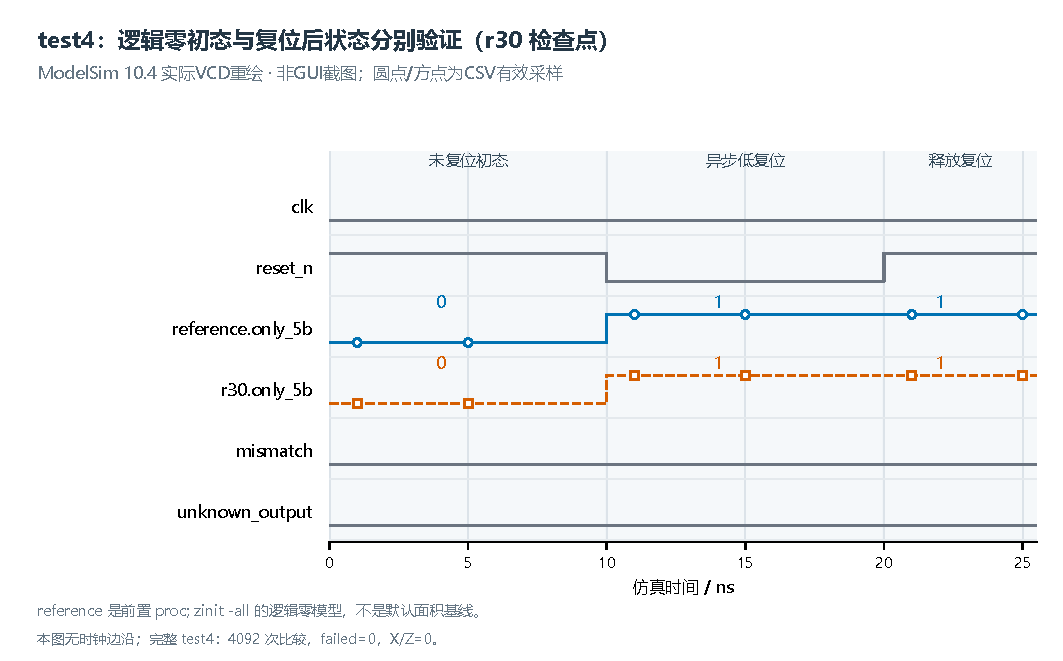
\includegraphics[width=14.4cm]{images/modelsim_zero_init.pdf}
\par\vspace{4pt}{\fontsize{10.5}{15.75}\selectfont 图8  当前test4无复位无边沿初态与异步复位观察\par}
\end{minipage}\end{center}
图8的1、5ns采样时reset\_\allowbreak{}n=1、clk=0，两侧only\_\allowbreak{}5b=0；11、15ns仅断言异步低复位，两侧为1；21、25ns释放复位而尚无时钟边沿，输出保持1。正常向量从26ns开始，首个边沿为30ns。复位后输出1不能被误读为逻辑零初态。test4独立重放的4092条CSV与原次逐字节一致。

\begin{center}\begin{minipage}{\textwidth}\centering
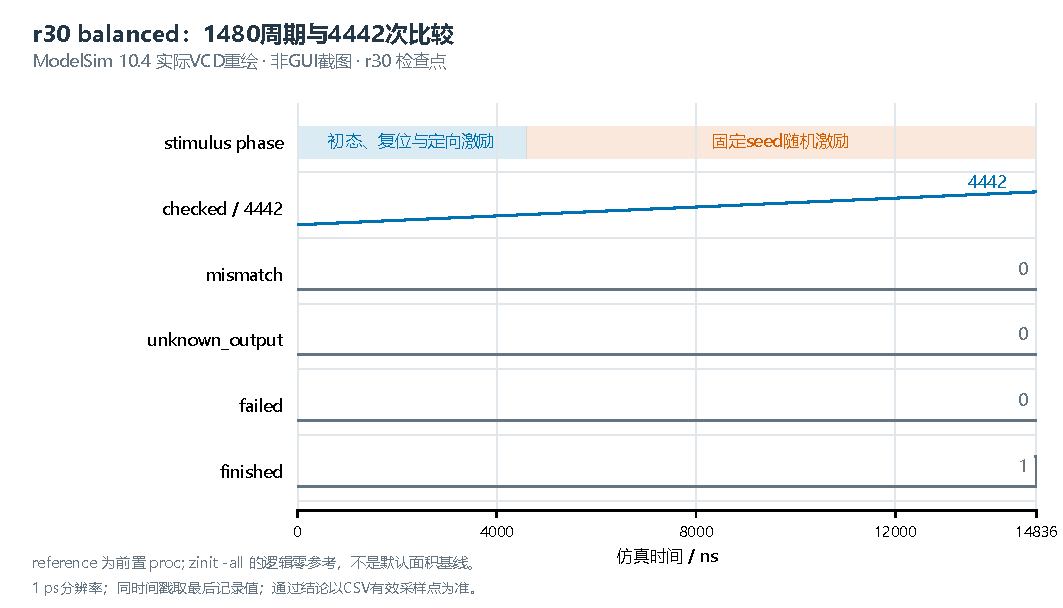
\includegraphics[width=14.4cm]{images/modelsim_zero_overview.pdf}
\par\vspace{4pt}{\fontsize{10.5}{15.75}\selectfont 图9  当前balanced全程激励阶段与检查计数\par}
\end{minipage}\end{center}
图9覆盖0—14836ns，显示初态、复位、定向激励与固定seed随机激励的先后阶段；checked最终为4442，failed与unknown保持0，finished在14826ns置1。该全程图用于定位记录范围，不能从压缩时间轴推断所有瞬态。

\begin{center}\begin{minipage}{\textwidth}\centering
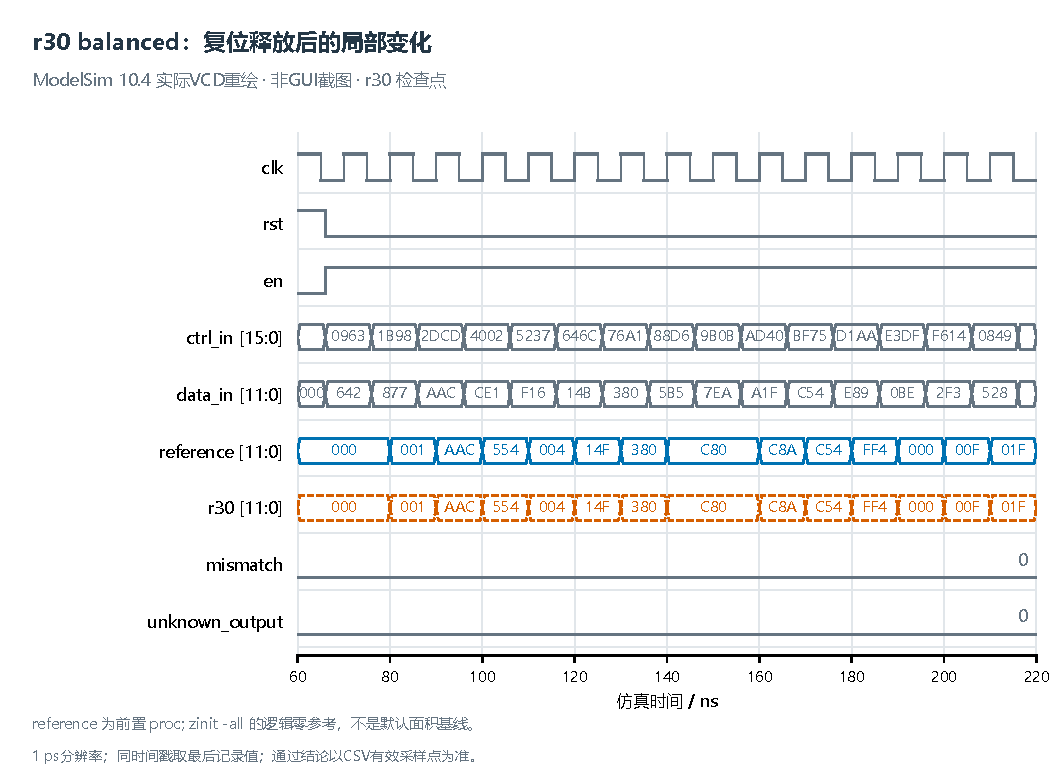
\includegraphics[width=14.4cm]{images/modelsim_zero_detail.pdf}
\par\vspace{4pt}{\fontsize{10.5}{15.75}\selectfont 图10  当前代表例局部数据变化与逐点输出比较\par}
\end{minipage}\end{center}
图10为60—220ns局部窗口，balanced于66ns撤销rst，采样输出依次为000、001、aac、554、004、14f、380等。蓝色实线表示同逻辑零初态参考，橙色虚线表示当前候选；data\_\allowbreak{}in仅展示原48位的低12位。

\begin{center}\begin{minipage}{\textwidth}\centering
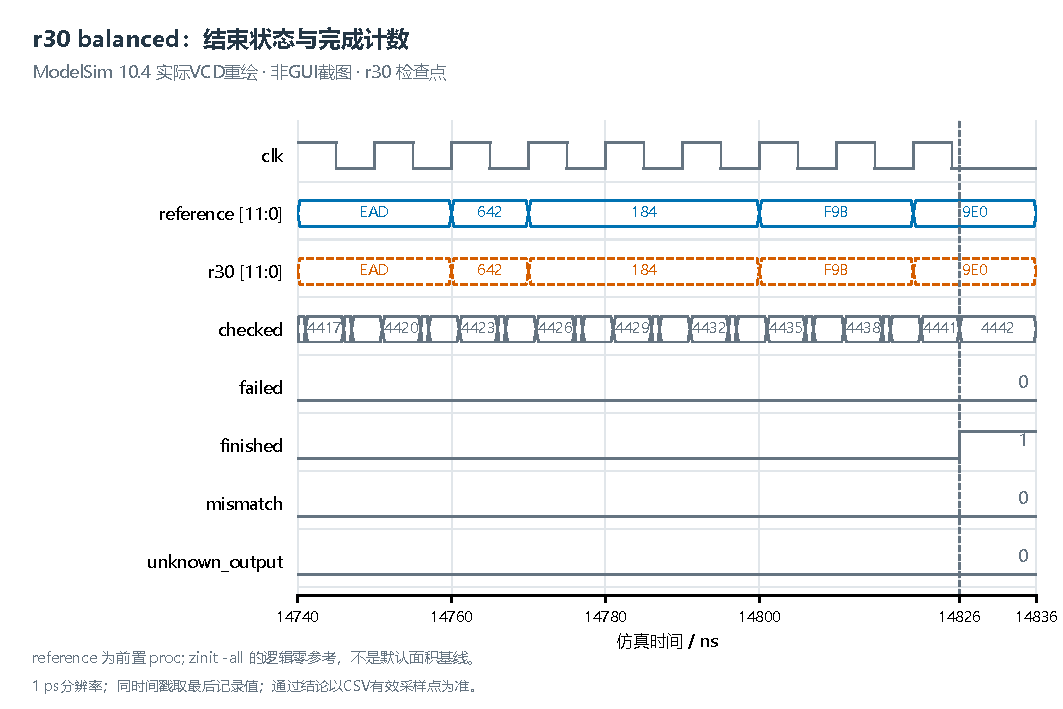
\includegraphics[width=14.4cm]{images/modelsim_zero_finish.pdf}
\par\vspace{4pt}{\fontsize{10.5}{15.75}\selectfont 图11  当前代表例结束窗口及比较计数\par}
\end{minipage}\end{center}
图11在14826ns显示finished=1、failed=0、checked=4442；两版末值均为9E0。该例共1480周期，seed=20261105。

图8—11来自r30\_\allowbreak{}native\_\allowbreak{}sload当前ModelSim导出的真实VCD重绘，明确非GUI截图。图8所示6个隔离采样点及balanced全部4442条采样输出已再次与VCD核对。test4其他周期边界可能先采样再更新异步复位，同时间戳VCD末值不必等于较早delta的CSV值；判错采用CSV有效采样。参考侧不是原默认面积基线。

\Needspace{129.6pt}\subsubsection*{test3：使能约束下的可观察状态}
\begin{center}\begin{minipage}{\textwidth}\centering
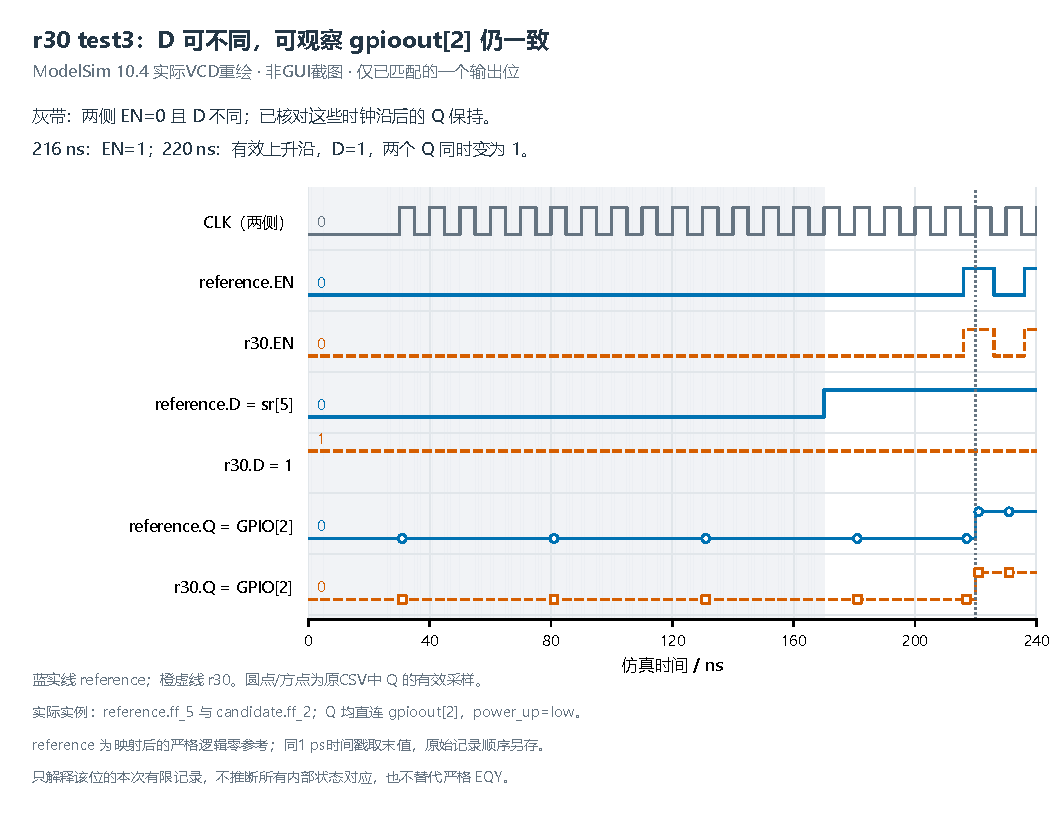
\includegraphics[width=14.4cm]{images/modelsim_observable.pdf}
\par\vspace{4pt}{\fontsize{10.5}{15.75}\selectfont 图12  test3未使能D可异、可观察Q保持的实测示例\par}
\end{minipage}\end{center}
r30 test3 的可观察状态示例（gpioout[2]）。本图由冻结 ModelSim 10.4 运行的实际 VCD 重绘，非 GUI 截图。参考端为经 proc; zinit -all 建立严格逻辑零语义后映射的网表，并非原 RTL 的直接事件仿真。JSON、转换后 Verilog 和 VCD 层级共同确认：reference.ff\_\allowbreak{}5（gpioout\_\allowbreak{}dffeas\_\allowbreak{}q\_\allowbreak{}2）与 candidate.ff\_\allowbreak{}2（gpioout\_\allowbreak{}dffeas\_\allowbreak{}q\_\allowbreak{}1）的 Q 均无反相地直连 gpioout[2]，power\_\allowbreak{}up 均为 low；参考 D=sr[5]，候选 D=1。灰带中两侧 EN=0 而 D 不同，所记录时钟上升沿后的 Q 保持；216 ns 两侧 EN 置 1，220 ns 上升沿采样 D=1 后，两侧 Q 同时变为 1。

完整记录中的 1354 个上升沿逐沿通过状态转移核验，其中 685 个沿为 EN=0 且 D 不同；26 个使能沿均采样相等 D。原 test3 的 4064 个有效 CSV 样本中，该位的两端 Q 与记录相符。圆点和方点标示图内选取的有效采样。图线以每个 1 ps 时间戳的最后记录值绘制，原始 VCD 记录顺序和逐时刻/\allowbreak{}逐沿检查表另存；不以 VCD 序列化顺序推断 delta 调度或无毛刺。结论仅限该可核实输出位和本次有限记录，不将所有内部名称视作对应状态，也不替代严格 EQY。

\Needspace{129.6pt}\subsubsection*{pipeline：保持控制与复位优先级}
\begin{center}\begin{minipage}{\textwidth}\centering
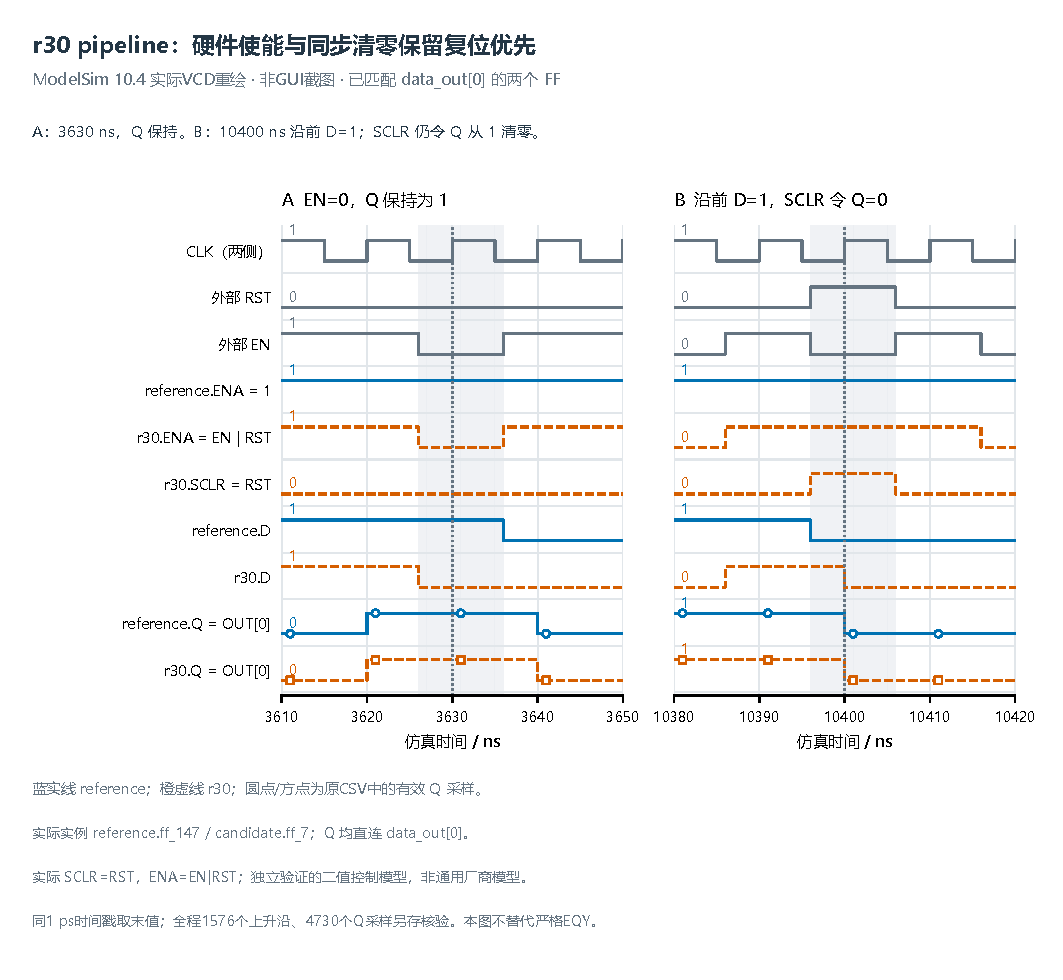
\includegraphics[width=14.4cm]{images/modelsim_sampling_boundary.pdf}
\par\vspace{4pt}{\fontsize{10.5}{15.75}\selectfont 图13  pipeline实际ENA关系及保持、复位的两个窗口\par}
\end{minipage}\end{center}
r30 pipeline 采样边界的真实有限记录。两侧 FF 的 Q 经 JSON、转换后 Verilog 与 VCD 层级核实，均直接驱动 data\_\allowbreak{}out[0]。参考端 24 个 FF 的 ENA 均为 1；r30 的 24 个 FF 共用一个实际 LUT 实现的 EN|RST。未增加寄存器或时钟级。A图3630 ns上升沿前，EN=RST=0，参考D=Q=1，候选D=0但ENA=0，两个Q均保持1。B图10400 ns上升沿前，RST=1且EN=0，候选ENA=1、SCLR=1；虽然候选D=1，Q仍从1清零，与参考Q一致，保持原复位优先。参考D因外部复位选择而为0，SCLR恒0。

全程1576个上升沿逐沿核对状态转移，其中242个沿为EN=RST=0且两侧D不同；7个沿为RST=1且外部EN=0。全部4730个CSV采样的该位Q与VCD相符。灰带标出对应控制条件；圆/\allowbreak{}方点是有效采样。两图来自本次ModelSim真实VCD，非GUI截图；每个1ps时间戳采用末记录值，原始记录顺序另存，不把序列化顺序当作delta调度。参考端经proc;zinit建立源逻辑零语义后映射，并非原RTL直接事件仿真，也不是默认面积基线。仿真FF使用经独立单步SAT与真实时钟归纳验证的受限SCLR/\allowbreak{}SLOAD扩展模型，实际SCLR/\allowbreak{}SLOAD/\allowbreak{}ASDATA原样连接；新域限定CLRN/\allowbreak{}PRN=1、ALOAD=0，旧异步清零域保留原行为。全部逐沿核验包含SLOAD选择ASDATA，器件全局控制按正常工作条件。该模型只承诺二值控制契约，不是通用厂商原语模型。本图仅说明这一对应位的有限记录，不能代替完整EQY或推导硬件延迟、无毛刺、全局内部状态等价。

\Needspace{129.6pt}\subsubsection*{pipeline：同步装载对实际数据来源的选择}
\begin{center}\begin{minipage}{\textwidth}\centering
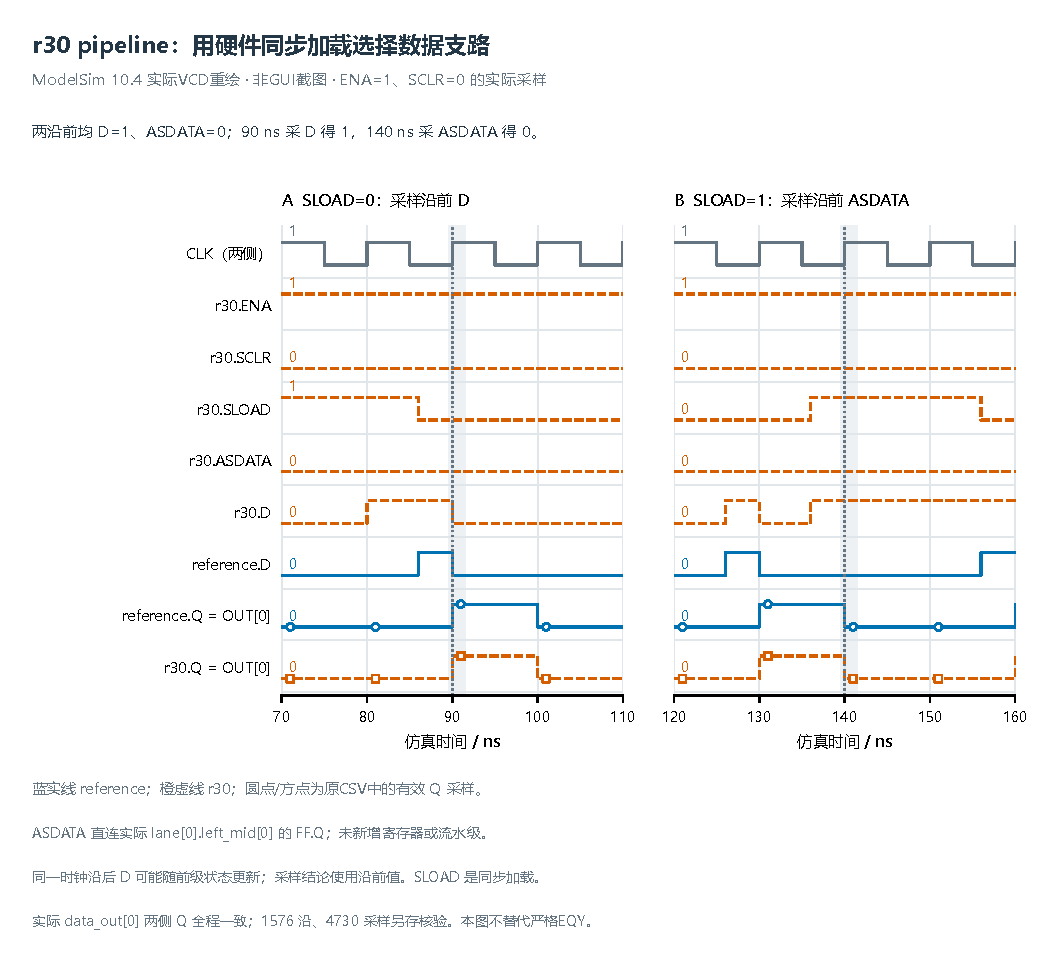
\includegraphics[width=14.4cm]{images/modelsim_sload_selection.pdf}
\par\vspace{4pt}{\fontsize{10.5}{15.75}\selectfont 图14  SLOAD=0取D、SLOAD=1取ASDATA的实际采样窗口\par}
\end{minipage}\end{center}
r30 的实际同步加载机制。A图90 ns沿前ENA=1、SCLR=0、SLOAD=0、D=1、ASDATA=0，Q从0变1；B图140 ns沿前ENA=1、SCLR=0、SLOAD=1、D=1、ASDATA=0，Q从1变0。两侧可观察data\_\allowbreak{}out[0]始终相等。实际候选zero\_\allowbreak{}pmux\_\allowbreak{}case02\_\allowbreak{}pipeline\_\allowbreak{}tb.candidate.ff\_\allowbreak{}7的ASDATA直接连接lane[0].left\_\allowbreak{}mid\_\allowbreak{}dffeas\_\allowbreak{}q\_\allowbreak{}1的Q，即lane[0].left\_\allowbreak{}mid[0]；沿前值是前一级原有状态，不新增寄存器或延迟。

全程433个使能且未清零的上升沿出现D与ASDATA不同，全部按实际SLOAD选择并逐沿核验。D可在同一上升沿后随前级状态更新，图中采用每个1ps时间戳末值；采样判定使用严格早于该沿的值。原VCD标量顺序、全部时间戳、1576条逐沿记录与4730个CSV该位采样位于pipeline\_\allowbreak{}boundary\_\allowbreak{}figure并由独立解析实现检查。仿真使用独立验证的受限二值控制模型；保持原十个端口及实际SCLR/\allowbreak{}SLOAD/\allowbreak{}ASDATA，器件全局控制按正常工作条件。本图由新r30真实ModelSim记录重绘，非GUI截图；不是厂家完整门级/\allowbreak{}时序仿真，也不替代完整形式等价证明。

本书波形由当次真实ModelSim导出的VCD重绘，并标注非GUI截图；原WLF、VCD、CSV、激励与工具日志保留。test4初态图使用六个隔离前导点，分别观察无时钟边沿的初态、复位断言及释放，正常周期激励随后开始。绘图取同时间戳最终记录值，判错以规定采样点CSV为准；有限仿真不证明delta-cycle无毛刺或真实器件时序。

\Needspace{129.6pt}\subsubsection*{3.3.2  接近千节点的独立规模验证}
补充样例将四份原模块以默认参数装入同一wrapper，保留193位外部输入、43位原输出和四个自由时钟。节点按实际最终映射叶单元计数：原版957、候选653，不按RTL位宽推算或凑成1000。它不是第十个官方用例，不进入九例面积均值。

\Needspace{165.0pt}
{\setstretch{1.0}\fontsize{10.5}{15.75}\selectfont
\begin{longtable}{>{\raggedright\arraybackslash}p{\dimexpr 0.416382\textwidth-2\tabcolsep\relax}>{\raggedright\arraybackslash}p{\dimexpr 0.291809\textwidth-2\tabcolsep\relax}>{\raggedright\arraybackslash}p{\dimexpr 0.291809\textwidth-2\tabcolsep\relax}}
\multicolumn{3}{c}{\normalsize 表12a  独立规模样例的资源与效率} \\[4pt]
\toprule
\bfseries 指标 & \bfseries 原默认基线 & \bfseries 当前候选 \\
\midrule
\endfirsthead
\multicolumn{3}{c}{\normalsize 表12a  独立规模样例的资源与效率（续）} \\[4pt]
\toprule
\bfseries 指标 & \bfseries 原默认基线 & \bfseries 当前候选 \\
\midrule
\endhead
\midrule\multicolumn{3}{r}{\small 续下页}\endfoot
\bottomrule\endlastfoot
最终映射叶单元 & 957 & 653 \\
LUT+标量取反 & 894 & 593 \\
DFF & 63 & 60 \\
墙钟/\allowbreak{}s & 0.7701572 & 0.6271899 \\
主进程峰值/\allowbreak{}字节 & 34697216 & 29573120 \\
\end{longtable}
}
该样例逻辑面积下降33.6689\%，时间比0.814366、内存比0.852320；两臂均低于60秒与2GB，本候选的相对两项均不超过1.05。原版预热10次后采用初始一对，未触发五对复测。计时只有read\_\allowbreak{}verilog及synth\_\allowbreak{}intel，使用其默认flatten；面积在全部计时后独立捕获。

完整EQY在同一分区证明全部43位原输出和20位附加状态关系，后者为联合证明目标而非assume。193位原输入中171位进入有效输出锥，其余原本未使用并自然消除；未新增输入约束。四个输入时钟的真实边沿由clk2fflogic保留。候选归一化无zinit或setundef，60个状态的power\_\allowbreak{}up均明确，其中59个low、1个high。

旧954节点记录采用额外前置hierarchy/\allowbreak{}flatten，与本轮默认综合流程不同，不能把两次数字相减当作版本收益。当前成功批次、端点哈希和归纳证明单独保存；前轮预检记录保留在其各自版本目录，不改写成本次执行。这个957节点实例给出原题规模界限内的客观实测，不能推出所有不超过1000节点的电路都已验证。

\Needspace{129.6pt}\subsubsection*{3.3.3  复现及证据检查}
复核顺序为：先核对版本和SHA-256，再确认原始九例与默认参数；检查默认脚本、两处内置调用和实际ABC路径；读逐例面积、同次效率和复测政策；最后检查源到候选的完整证明、初始化审计及当次ModelSim记录。任何二进制或源码修改都需要重新绑定相应结果，不以旧版本通过替代新端点验证。

可迁移运行文件取自当前候选的冻结安装目录，程序SHA-256与正式测量一致；源码取自对应候选快照。持续研发的共享构建目录可能已是后续试验版本，不能直接复制它覆盖当前交付程序。

r20迁移首先完成含空格目录下的test4不计时捕获与直接EQY启动检查。其后的首次完整All批次中，九例测量和端点绑定通过，但4个长名用例因Windows未规约路径过长出现工具读取ERROR，另5例证明通过；原失败目录与报告保留，不能将这4项错误解释为PASS或逻辑反例。

路径修复后的r20新完整All批次通过PowerShell入口重新完成九例v3计时、独立面积与端点捕获，以及无候选补初值的九例完整EQY，退出码0、全部客观检查通过。证明在独立短目录运行，443个文件原样归档，完成时原目录、归档和清单的文件集合及SHA逐一相同。

\Needspace{5\baselineskip}
{\small
\noindent\begin{minipage}{\linewidth}
\begin{verbatim}
RELOCATION_FIXED2_AUDIT.json
SHA-256:
abfe853ca672a5a32da7133d22acf47c519e459526c58abc2a6c49accedf4b8d
\end{verbatim}
\end{minipage}
\par}
全部持久归档已逐文件重新核对；部分TEMP源文件当前已不可复核，不据此改写当时记录。此批次为r20历史路径修复证据，不替换当前候选主表，也不改名为当前候选运行。

当前r30\_\allowbreak{}native\_\allowbreak{}sload另在含空格的迁移目录，经现有PowerShell 7入口实际完成一次完整All：28个计时进程（含预热），未触发复核；全部计时结束后捕获面积与端点，再直接证明九例源逻辑0到实际候选，九例完整EQY均通过，退出码0。面积均值与主表相同；本迁移批次最大时间比0.985661、内存比1.010402，均不超过1.05。该独立复现批次不替换主表正式批次，不据两次时间差推断算法收益。

迁移前后5157项包文件及5154项原始路径映射保持，443份证明文件在完成时由短执行目录逐字节核对后归档，持久归档亦经逐文件复核。路径预检最大205个UTF-16单位，小于240。该迁移审计覆盖冻结程序和证据包，项目书未列入当次验收范围。

\Needspace{5\baselineskip}
{\small
\noindent\begin{minipage}{\linewidth}
\begin{verbatim}
RELOCATION_R30_ALL_AUDIT.json
SHA-256:
514c67ad3dff78a6faccc9cdf506b4bbefb730ca3fa595676614fd41e5e59b25
\end{verbatim}
\end{minipage}
\par}
R30迁移前保留两项准备错误：生成脚本时旧header匹配条件不合，以及把波形ZIP条目误当成原目录文件全集。后者逐项确认ZIP内365项字节相同，目录另有200项受限ModelSim缓存和transcript；未删除或刷新stage。两项均未进入All，修正准备检查后实际只运行上述一次All。历史r23的Python Store别名取哈希与Windows PowerShell 5.1策略异常另存，不算作本次R30启动失败。全程未修改系统执行策略。

使用时在PowerShell 7终端进入包目录，直接运行Run-OfficialTests.ps1；不要切换到Windows PowerShell 5.1，也不以修改执行策略或Bypass参数处理启动问题。入口只设置子进程ABC/\allowbreak{}PATH。源码重建助手使用当前PowerShell 7另起子进程；这项启动修正不代表本轮已重新编译程序，重建后仍须另做完整验证。

\Needspace{211.0pt}
{\setstretch{1.0}\fontsize{10.5}{15.75}\selectfont
\begin{longtable}{>{\raggedright\arraybackslash}p{\dimexpr 0.218430\textwidth-2\tabcolsep\relax}>{\raggedright\arraybackslash}p{\dimexpr 0.375427\textwidth-2\tabcolsep\relax}>{\raggedright\arraybackslash}p{\dimexpr 0.406143\textwidth-2\tabcolsep\relax}}
\multicolumn{3}{c}{\normalsize 表13  交付材料及复核重点} \\[4pt]
\toprule
\bfseries 材料 & \bfseries 内容 & \bfseries 重点 \\
\midrule
\endfirsthead
\multicolumn{3}{c}{\normalsize 表13  交付材料及复核重点（续）} \\[4pt]
\toprule
\bfseries 材料 & \bfseries 内容 & \bfseries 重点 \\
\midrule
\endhead
\midrule\multicolumn{3}{r}{\small 续下页}\endfoot
\bottomrule\endlastfoot
baseline /\allowbreak{} optimized & 原默认基线、候选程序、依赖及入口 & 使用同一ABC；入口负责配置路径 \\
source /\allowbreak{} cases & 当前源码、原始九例和默认参数 & 无用例名特判；参数不覆盖 \\
proof /\allowbreak{} evidence & 源逻辑0证明、端点与测量报告 & 原始角色名称与实际端点对应 \\
ModelSim证据 & r30\_\allowbreak{}modelsim：WLF/\allowbreak{}VCD/\allowbreak{}CSV、图及重放脚本 & 本次七图由新VCD生成；有限采样，非GUI截图 \\
project\_\allowbreak{}book & Word、LaTeX、PDF、图源和短对照报告 & 表图与同一冻结报告对应 \\
\end{longtable}
}
\clearpage
\Needspace{184.6pt}\section*{第四部分  总结}
\Needspace{129.6pt}\subsection*{4.1  可扩展之处}
下一步验证应沿明确边界展开：补充更多RAM类型和锁存器前，先定义可支持的初始化行为与失败策略；开展更大规模或不同参数测试时，独立记录输入、完整证明及性能。对控制恢复、bank、算术、DAG和ROM规则开展固定工具链下的消融，才有依据区分各模块贡献。当前九例成功不能外推全部设计。

公开提交构建、原默认面积基线和源逻辑初态参考应持续分离。若获得官方完整补丁，应在相同政策下重建、重测、重证；不能仅替换版本字符串。为适应更严苛效率条件，优化应减少自定义pass的无效扫描和重复构图，同时保持通用结构判断，不能通过绕过其他综合步骤获得表面加速。

\Needspace{129.6pt}\subsection*{4.2  心得体会}
本项目的主要经验来自反例：逻辑0与物理0不一定是同一个状态，晚补初值也不一定能找回早已删除的历史。把初始化声明放到顺序变换之前，让实际产物承担契约，再从源直接验证，才能使“通过”与交付行为对应。保留旧反例和未证出的中间记录，比只展示成功状态更有助于说明方法边界。

当前绑定候选的面积均值为36.2522\%，v3 两命令逐例效率结论为逐例均不超过1.05，完整源逻辑零证明九例通过。成果由内置程序、固定用例、同次测量和可追溯端点共同构成；不是任意初态强等价、理论最优或满分承诺。

\clearpage
\Needspace{129.6pt}\section*{第五部分  参考文献}
\begin{samepage}
{\setstretch{1.0}\fontsize{10.5}{15.75}\selectfont
\noindent\hangindent=2em [1] 赛事主办方. FPGA创新赛道赛题：选题二，多路选择器PMUX结构优化[Z]. 用户提供原题PDF，印刷页4—6（PDF第6—8页）；文件SHA-256见证据清单，2026.
\par
}
\end{samepage}
\begin{samepage}
{\setstretch{1.0}\fontsize{10.5}{15.75}\selectfont
\noindent\hangindent=2em [2] FPGA创新大赛问题汇总[Z]. 用户提供工作簿，Sheet1答复列C；最新日期组2026.10.27—10.30. 本文按答复单元格逐项引用，发布方身份未另行认证.
\par
}
\end{samepage}
\begin{samepage}
{\setstretch{1.0}\fontsize{10.5}{15.75}\selectfont
\noindent\hangindent=2em [3] YosysHQ. Yosys Open SYnthesis Suite: Documentation[EB/\allowbreak{}OL]. [2026-11-01]. \url{https://yosyshq.readthedocs.io/projects/yosys/en/latest/}.
\par
}
\end{samepage}
\begin{samepage}
{\setstretch{1.0}\fontsize{10.5}{15.75}\selectfont
\noindent\hangindent=2em [4] YosysHQ. Optimization passes: Yosys Documentation[EB/\allowbreak{}OL]. [2026-11-01]. \url{https://yosyshq.readthedocs.io/projects/yosys/en/latest/using_yosys/synthesis/opt.html}.
\par
}
\end{samepage}
\begin{samepage}
{\setstretch{1.0}\fontsize{10.5}{15.75}\selectfont
\noindent\hangindent=2em [5] YosysHQ. EQY Documentation[EB/\allowbreak{}OL]. [2026-11-01]. \url{https://yosyshq.readthedocs.io/projects/eqy/en/latest/}.
\par
}
\end{samepage}
\begin{samepage}
{\setstretch{1.0}\fontsize{10.5}{15.75}\selectfont
\noindent\hangindent=2em [6] YosysHQ. Equivalence and X-Propagation: EQY Documentation[EB/\allowbreak{}OL]. [2026-11-01]. \url{https://yosyshq.readthedocs.io/projects/eqy/en/latest/xprop.html}.
\par
}
\end{samepage}
\begin{samepage}
{\setstretch{1.0}\fontsize{10.5}{15.75}\selectfont
\noindent\hangindent=2em [7] BRAYTON R, MISHCHENKO A. ABC: An Academic Industrial-Strength Verification Tool[C]/\allowbreak{}/\allowbreak{}Computer Aided Verification. LNCS 6174. Springer, 2010: 24-40. \url{https://doi.org/10.1007/978-3-642-14295-6_5}.
\par
}
\end{samepage}
\begin{samepage}
{\setstretch{1.0}\fontsize{10.5}{15.75}\selectfont
\noindent\hangindent=2em [8] BRYANT R E. Graph-Based Algorithms for Boolean Function Manipulation[J]. IEEE Transactions on Computers, 1986, C-35(8): 677-691. \url{https://doi.org/10.1109/TC.1986.1676819}.
\par
}
\end{samepage}
\begin{samepage}
{\setstretch{1.0}\fontsize{10.5}{15.75}\selectfont
\noindent\hangindent=2em [9] 本项目组. 逻辑零初态版本的冻结实测、形式证明与仿真材料[DS]. 2026-11-01. \texttt{binding.\allowbreak{}json}；proof/\allowbreak{}\texttt{report.\allowbreak{}json}；performance/\allowbreak{}\texttt{report.\allowbreak{}json}；\texttt{simulation\_\allowbreak{}report.\allowbreak{}json}. 各文件版本、原始路径与SHA-256见交付清单.
\par
}
\end{samepage}
\begin{samepage}
{\setstretch{1.0}\fontsize{10.5}{15.75}\selectfont
\noindent\hangindent=2em [10] Altera. Quartus Prime Pro Edition User Guide, 25.1: 2.5.2 Secondary Register Control Signals Such as Clear and Clock Enable[EB/\allowbreak{}OL]. 2026-05-13 [2026-11-02]. \url{https://docs.altera.com/r/docs/683082/25.1/quartus-prime-pro-edition-user-guide/secondary-register-control-signals-such-as-clear-and-clock-enable}.
\par
}
\end{samepage}
\begin{samepage}
{\setstretch{1.0}\fontsize{10.5}{15.75}\selectfont
\noindent\hangindent=2em [11] Altera. Cyclone IV Device Handbook, Volume 1: Chapter 2, Logic Elements and Logic Array Blocks in Cyclone IV Devices[M/\allowbreak{}OL]. 2009-11: 2–6—2–7 [2026-11-02]. \url{https://docs.altera.com/api/khub/documents/3srzmTgxxMHVsaxzQUGqXg/content}.
\par
}
\end{samepage}
\end{document}
